\documentclass[a4paper,12pt]{report}
\usepackage[utf8]{inputenc}
\usepackage[spanish]{babel}
\usepackage{amsmath}
\usepackage{makecell}
\usepackage{amsfonts}
\usepackage{amssymb}
\usepackage{multirow}
%\usepackage{makeidx}
\usepackage{graphicx}
\usepackage{fancyhdr}
\usepackage{hyperref}
\usepackage{float}
\usepackage{enumerate}
\usepackage[toc,page]{appendix}
\usepackage[nottoc]{tocbibind}
\usepackage{color}
\usepackage[dvipsnames]{xcolor}
\usepackage{tabularx}
\definecolor{gray97}{gray}{.97}
\definecolor{gray75}{gray}{.75}
\definecolor{gray45}{gray}{.45}
\usepackage{listings}
\lstset{ frame=Ltb,
     framerule=0pt,
     aboveskip=0.5cm,
     framextopmargin=3pt,
     framexbottommargin=3pt,
     framexleftmargin=0.4cm,
     framesep=0pt,
     rulesep=.4pt,
     backgroundcolor=\color{gray97},
     rulesepcolor=\color{black},
     %
     stringstyle=\ttfamily,
     showstringspaces = false,
     basicstyle=\small\ttfamily,
     commentstyle=\color{gray45},
     keywordstyle=\bfseries,
     %
     numbers=left,
     numbersep=15pt,
     numberstyle=\tiny,
     numberfirstline = false,
     breaklines=true,
   }
 
% minimizar fragmentado de listados
\lstnewenvironment{listing}[1][]
   {\lstset{#1}\pagebreak[0]}{\pagebreak[0]}
 
\lstdefinestyle{consola}
   {basicstyle=\scriptsize\bf\ttfamily,
    backgroundcolor=\color{gray75},
   }
 
\lstdefinestyle{C}
   {language=C,
   }
\usepackage[top=2cm]{geometry}
\pretolerance=2000
\tolerance=3000
\begin{document}

\begin{titlepage}
\begin{sffamily}
\color{NavyBlue}
\begin{center}
%\vspace*{-1cm}
\begin{figure}[htb]
\begin{center}
\vspace*{0.6cm}

\includegraphics[width=15cm]{figures/logoEHU_blanco_mediano.eps}
\vspace*{1.6cm}
\end{center}
\end{figure}
\begin{LARGE}
Máster Universitario en Modelización e Investigación Matemática, Estadística y Computación 
2023/2024 \\%indicar el curso académico
\vspace*{1cm}
\textsl{Trabajo Fin de Máster}\\
\end{LARGE}
\Huge{\textbf{Título del trabajo}} %Más significativo que el anterior
\vspace*{1cm}
\rule{80mm}{0.1mm}\\
\huge{Alexander de la Puente González}\\ %Separar cada autor con \\ 
\vspace*{0.5cm}
\begin{Large}
Director/es\\
Josu Doncel Vicente\\
Nombre Apellido1 Apellido2\\
Lugar y fecha de presentación prevista\\
\end{Large}
\end{center}
\end{sffamily}
\end{titlepage}

%\frontmatter
\pagestyle{fancy}
\fancyhead{} % Clear all header fields
\setlength\headheight{21.2pt}
\rhead{\color{NavyBlue} Mi encabezado} %Poner encabezado

\renewcommand{\tablename}{\textbf{Tabla}} %para poner la palabra en mayusucula
\renewcommand{\figurename}{\textbf{Figura}} % para poner la palabra en mayuscula
\renewcommand{\listtablename}{Índice de tablas}

\title{}
\date{}
\maketitle


\clearpage
\pagenumbering{Roman}
\setcounter{page}{1}

\tableofcontents
%\thispagestyle{empty}

\listoffigures
%\thispagestyle{empty}

\listoftables
%\thispagestyle{empty}

%Para imagenes
%\begin{figure}[H]
%\centering
%\includegraphics[scale=0.8]{imagenes/*.png}
%\caption{}
%\end{figure}

%\mainmatter
\clearpage
\pagenumbering{arabic}
\setcounter{page}{1}

%Comenzar el trabajo

\chapter{Introducción}

\begin{itemize}

\item Contextualización del problema.

\item Antecedentes y citas a trabajos (libros, artículos o manuscritos) que sirven de referencia, como por ejemplo \cite{DindosPipherRule2016}

\item Relación con el contenido de alguna/s asignatura/s del máster y técnicas o tería utilizadas en el planteamiento o resolución del problema.

\item Comentario sobre los capítulos o secciones que componen la memoria.

\end{itemize}

\section{Contextualización del problema}

En los últimos años, el uso de estrategias de trading automatizadas ha cobrado una gran relevancia en el mundo financiero. La incorporación de 
técnicas de aprendizaje profundo y métodos avanzados de análisis financiero ha permitido el desarrollo de estrategias más sofisticadas y eficientes. 
En este contexto, la aplicación de Reinforcement Learning (RL) y metodologías avanzadas, como las propuestas por Marcos López de Prado, ofrecen un 
enfoque novedoso para abordar los desafíos del trading financiero.


% \section{Antecedentes}

% Diversos estudios y trabajos han explorado la aplicación de RL en finanzas. Por ejemplo, Dindos y Pipher (\cite{DindosPipherRule2016}) 
% demostraron la viabilidad de usar RL para optimizar portafolios financieros. Además, López de Prado en su libro 
% "Advances in Financial Machine Learning" proporciona una guía exhaustiva sobre técnicas avanzadas de machine learning aplicadas a finanzas, 
% que sirven como base para este trabajo.

\section{Relación con el contenido del máster}

Este trabajo se relaciona estrechamente con varias asignaturas del máster, como la teoría de machine learning, optimización y finanzas 
cuantitativas. Las técnicas de deep RL, así como las metodologías avanzadas de análisis financiero, son fundamentales para la formulación 
y resolución del problema planteado.

\section{Estructura del documento}

El presente trabajo se estructura en los siguientes capítulos:

\begin{itemize}
    \item \textbf{Capítulo 1: Introducción} - Se presenta el contexto del problema, los antecedentes relevantes y la relación con los 
    contenidos del máster.
    \item \textbf{Capítulo 2: Planteamiento del problema y formulación} - Se detalla el problema a resolver, incluyendo la formulación 
    matemática y los objetivos específicos.
    \item \textbf{Capítulo 3: Caso de estudio y simulaciones} - Se presenta un caso de estudio concreto, junto con las simulaciones y 
    resultados obtenidos.
    \item \textbf{Capítulo 4: Conclusiones} - Se resumen los hallazgos principales y se discuten posibles trabajos futuros.
\end{itemize}

\chapter{Estado del arte ???}

\chapter{Planteamiento del problema y formulación}
\section{Descripción de los Datos Financieros}

Aunque los datos financieros vienen en muchas formas, este trabajo se centrará en aquellos provenientes de acciones o índices 
(cestas de instrumentos financieros). Para simplificar, en lugar de pensar en instrumentos financieros individuales, consideraremos 
la serie temporal subyacente de precios.

\subsection{Introducción a la Serie Temporal}

La serie temporal $\{p_t\}$ representa el precio de una acción o índice en el instante de tiempo discreto $t$. Es importante 
notar que $t$ dependerá de la frecuencia de muestreo utilizada para recopilar los datos.

\subsubsection{Frecuencia}

\begin{itemize}
    \item \textbf{Datos de Baja Frecuencia (LF)}: Diarios, mensuales, trimestrales.
    \item \textbf{Datos de Alta Frecuencia (HF)}: Intradía (30 min., 5 min., etc.).
\end{itemize}

Al introducir estos conceptos, es pertinente señalar que el modelado en finanzas se realiza con el logaritmo natural del precio 
(log-precios) en lugar de los precios regulares. Esto se representará como $y_t := \log(p_t)$. Para ilustrar esto, se 
introduce el simple, pero ampliamente utilizado, modelo de un paseo aleatorio con deriva:

\[
y_t = y_{t-1} + \mu + \epsilon_t
\]

donde $\epsilon_t \sim i.i.d. \mathcal{N}(0, \sigma^2)$.

\subsection{Retornos de Activos}

El siguiente concepto a introducir son los retornos, una técnica para normalizar los precios y permitir la comparación 
entre diferentes series temporales, independientemente del valor del precio. Los dos tipos que se van a utilizar son 
los retornos lineales y logarítmicos.

\begin{itemize}
    \item \textbf{Lineales}: $R_t := \frac{p_t - p_{t-1}}{p_{t-1}} = \frac{p_t}{p_{t-1}} - 1$
    \item \textbf{Logarítmicos}: $r_t := \log\left(\frac{p_t}{p_{t-1}}\right) = \log(p_t) - \log(p_{t-1}) = y_t - y_{t-1}$
\end{itemize}

Propiedades destacadas:

\begin{enumerate}
    \item $r_t = \log(1 + R_t)$
    \item La serie de Taylor de $\log(1 + x) = \sum_{k=1}^{\infty} \frac{(-1)^{k+1} x^k}{k}$ da como resultado $r_t 
    \approx R_t$ cuando $R_t \approx 0$.
    \item Retornos lineales compuestos:

    \[
    R_t(k) := \frac{p_t - p_{t-k}}{p_{t-k}} = \frac{p_t}{p_{t-k}} - 1 = \left(1 + R_t\right) \cdot \left(1 + R_{t-1}\right) 
    \cdots \left(1 + R_{t-(k-1)}\right) - 1
    \]

    \item Retornos logarítmicos compuestos:

    \[
    r_t(k) := \log\left(\frac{p_t}{p_{t-k}}\right) = y_t - y_{t-k} = (y_t - y_{t-1}) + \cdots + (y_{t-(k-1)} - 
    y_{t-k}) = r_t + \cdots + r_{t-(k-1)}
    \]
\end{enumerate}




\begin{figure}[H]
    \centering
    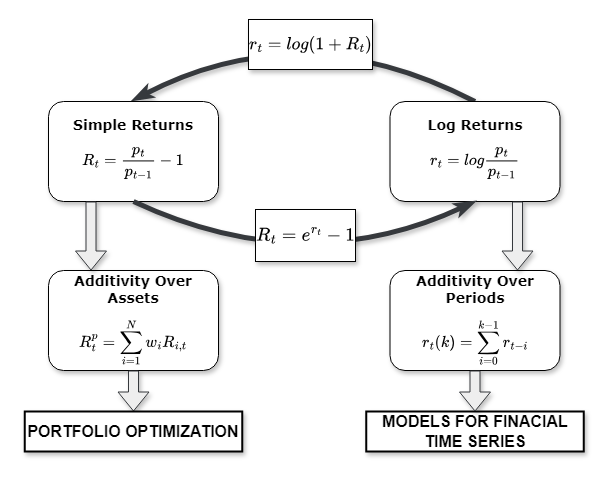
\includegraphics[width=0.8\textwidth]{figures/simple_and_log_ret_relation.png}
    \caption{ola}
    \label{fig:log-returns}
\end{figure}


% Para mostrar lo que se ha definido, se presentan en las figuras \ref{fig:log-returns} y \ref{fig:log-prices} los log-retornos y log-precios del índice S&P500 para el periodo que abarca del 01-01-2015 al 01-10-2018.

% \begin{figure}[H]
%     \centering
%     \includegraphics[width=0.8\textwidth]{log-returns.png}
%     \caption{Log-Returns del S&P500}
%     \label{fig:log-returns}
% \end{figure}

% \begin{figure}[H]
%     \centering
%     \includegraphics[width=0.8\textwidth]{log-prices.png}
%     \caption{Log-Prices del S&P500}
%     \label{fig:log-prices}
% \end{figure}

\section{Hechos Estilizados}

Los hechos estilizados son patrones o regularidades observadas empíricamente en los datos financieros que se 
presentan de manera consistente en diferentes mercados, periodos de tiempo y condiciones económicas. Estos hechos 
no dependen de modelos teóricos específicos, sino que se derivan directamente de la observación de los datos. La 
identificación de estos patrones es crucial para el desarrollo y validación de modelos financieros y econométricos. 
En este trabajo, nos basamos en los hechos estilizados descritos por Rama Cont (2001) en su artículo \textit{Empirical 
properties of asset returns: stylized facts and statistical issues} \cite{Cont2001}.

A continuación, se describen los principales hechos estilizados relevantes para este estudio:

\begin{enumerate}
    \item \textbf{Ausencia de Autocorrelaciones}: Los retornos de los activos financieros, especialmente en 
    frecuencias diarias y superiores, tienden a mostrar una autocorrelación lineal insignificante. Esto significa 
    que los retornos pasados no son buenos predictores de los retornos futuros, lo cual es consistente con la hipótesis 
    del mercado eficiente en su forma débil. Sin embargo, en escalas temporales intradía, pueden observarse autocorrelaciones significativas.
    \item \textbf{Colas Pesadas}: La distribución de los retornos de los activos financieros presenta colas más gruesas que una distribución 
    normal. Esto implica que los eventos extremos (grandes movimientos de precios) ocurren con mayor frecuencia de lo que se esperaría bajo 
    una distribución normal. Las colas pesadas se modelan mejor con distribuciones como la distribución de Pareto o la distribución t de Student.
    \item \textbf{Asimetría de Ganancias/Pérdidas}: Los retornos de los activos financieros muestran una asimetría en sus movimientos extremos. 
    Las caídas bruscas en los precios (pérdidas) son más comunes y pronunciadas que los incrementos bruscos (ganancias). Esto se debe a factores 
    como el pánico de los inversores y las ventas masivas en respuesta a malas noticias.
    \item \textbf{Gaussianidad Agregada}: A medida que se incrementa la escala temporal sobre la cual se calculan los retornos (por ejemplo, 
    pasando de retornos diarios a retornos mensuales), la distribución de los retornos tiende a aproximarse a una distribución normal. Esto es 
    consistente con el teorema central del límite, que establece que la suma de variables aleatorias independientes y con varianza finita tiende 
    hacia una distribución normal.
    \item \textbf{Intermitencia}: Los retornos financieros muestran una alta variabilidad en todas las escalas temporales. Esto significa que 
    los periodos de alta y baja volatilidad no están distribuidos uniformemente en el tiempo, sino que se alternan de manera impredecible.
    \item \textbf{Agrupamiento de Volatilidad}: La volatilidad de los retornos tiende a aparecer en clústeres. Periodos de alta volatilidad 
    tienden a ser seguidos por más periodos de alta volatilidad, y lo mismo ocurre con los periodos de baja volatilidad. Este fenómeno se 
    puede modelar mediante modelos de heterocedasticidad condicional, como los modelos GARCH (Generalized Autoregressive Conditional 
    Heteroskedasticity).
\end{enumerate}

Estos hechos estilizados proporcionan una base empírica sobre la cual se pueden construir y validar modelos financieros. La identificación 
y comprensión de estos patrones ayudan a mejorar la precisión de los modelos de riesgo, a desarrollar estrategias de trading más robustas 
y a diseñar mejores políticas de regulación financiera.


\subsection{Propiedades Estadísticas}

La autocorrelación de los log-retornos diarios se define como:

\[
\rho_k = \frac{\text{Cov}(r_t, r_{t+k})}{\sqrt{\text{Var}(r_t) \text{Var}(r_{t+k})}}
\]

donde $\text{Cov}(r_t, r_{t+k})$ es la covarianza de $r_t$ y $r_{t+k}$, y $\text{Var}(r_t)$ la varianza de $r_t$.

% En la figura \ref{fig:autocorrelations} se pueden observar las autocorrelaciones de los log-retornos diarios del S&P500. Por definición, $\rho_0 = 1$. Aparte de eso, el resto de lags son insignificantes o apenas superan el umbral significativo.

% \begin{figure}[H]
%     \centering
%     \includegraphics[width=0.8\textwidth]{autocorrelations.png}
%     \caption{Autocorrelaciones de los log-retornos diarios del S&P500}
%     \label{fig:autocorrelations}
% \end{figure}

% La figura \ref{fig:pdf-log-returns} muestra el histograma de los log-retornos diarios, semanales y mensuales del S&P500. Esto ilustra los hechos estilizados 2 y 4, mostrando claramente las colas pesadas y cómo evoluciona hacia una distribución normal a medida que aumenta la escala temporal de los retornos.

% \begin{figure}[H]
%     \centering
%     \includegraphics[width=0.8\textwidth]{pdf-log-returns.png}
%     \caption{Pdf ajustada a los log-retornos del S&P500}
%     \label{fig:pdf-log-returns}
% \end{figure}

% Finalmente, la figura \ref{fig:qq-plot} ilustra, a través de gráficos QQ (Quantile-Quantile), que los log-retornos no siguen una distribución normal. La curvatura en los extremos es un claro signo de una distribución de colas pesadas.

% \begin{figure}[H]
%     \centering
%     \includegraphics[width=0.8\textwidth]{qq-plot.png}
%     \caption{QQ Plots de los log-retornos del S&P500}
%     \label{fig:qq-plot}
% \end{figure}

\subsection{Datos de Alta Frecuencia}

Los datos de alta frecuencia (HF) representan el registro de precios y volúmenes de transacciones de activos financieros en intervalos 
de tiempo muy cortos, como segundos o milisegundos. Estos datos incluyen información detallada sobre cada transacción, como el precio, 
la cantidad negociada y el tiempo exacto de la transacción. A continuación, se detallan algunas características clave de los datos de 
alta frecuencia:

\begin{itemize}
    \item \textbf{Granularidad Temporal}: Los datos se registran en intervalos muy cortos, lo que permite un análisis detallado de la 
    dinámica del mercado en el corto plazo.
    \item \textbf{Volumen de Datos}: La gran cantidad de transacciones que ocurren en cortos periodos de tiempo genera volúmenes 
    masivos de datos que deben ser almacenados y procesados.
    \item \textbf{Precisión}: Incluyen información precisa sobre el precio y el volumen de cada transacción, así como el tiempo exacto 
    en que ocurrieron.
    \item \textbf{Eventos de Mercado}: Los datos de alta frecuencia capturan eventos de mercado que no son visibles en datos de menor 
    frecuencia, como órdenes de compra y venta, cambios en la profundidad del mercado y reacciones instantáneas a noticias.
\end{itemize}

A pesar de sus ventajas, los datos de alta frecuencia presentan varios desafíos:

\begin{itemize}
    \item \textbf{Costo y Accesibilidad}: Los datos de alta frecuencia son difíciles y costosos de obtener, ya que generalmente requieren 
    suscripciones a servicios de datos financieros especializados y costosos.
    \item \textbf{Procesamiento y Almacenamiento}: El volumen masivo de datos requiere infraestructuras avanzadas para su almacenamiento 
    y procesamiento eficiente.
    \item \textbf{Ruido y Volatilidad}: La alta granularidad temporal de estos datos incluye mucho ruido, lo que puede complicar el 
    análisis y modelado.
\end{itemize}

Debido a estos desafíos, en este trabajo se utilizarán datos de minuto. Los datos de minuto representan un compromiso entre la 
granularidad y la manejabilidad, proporcionando suficiente detalle para un análisis robusto sin los costos y complejidades asociados 
con los datos de alta frecuencia. Estos datos son más accesibles y permiten capturar las tendencias y patrones intradía sin la 
sobrecarga de procesamiento asociada con datos de mayor frecuencia.

% \begin{figure}[H]
%     \centering
%     \includegraphics[width=0.8\textwidth]{minute_data_example.png}
%     \caption{Ejemplo de Datos de Minuto}
%     \label{fig:minute-data-example}
% \end{figure}

\subsection{Datos Utilizados}

En este trabajo se utilizarán dos conjuntos de datos financieros: los datos de Bitcoin y los datos del SPY (SPDR S\&P 500 500 ETF Trust). 
A continuación, se describen estos datos, se muestran sus series temporales y se analizan sus propiedades estadísticas para verificar 
si cumplen con los hechos estilizados mencionados anteriormente.

\subsubsection{Datos de Bitcoin}

Bitcoin es una criptomoneda y un sistema de pago descentralizado que ha ganado popularidad y relevancia en los mercados financieros. 
Los datos de Bitcoin que utilizaremos incluyen los precios de cierre por minuto. A continuación se muestra la serie temporal de precios 
de Bitcoin:

\begin{figure}[H]
    \centering
    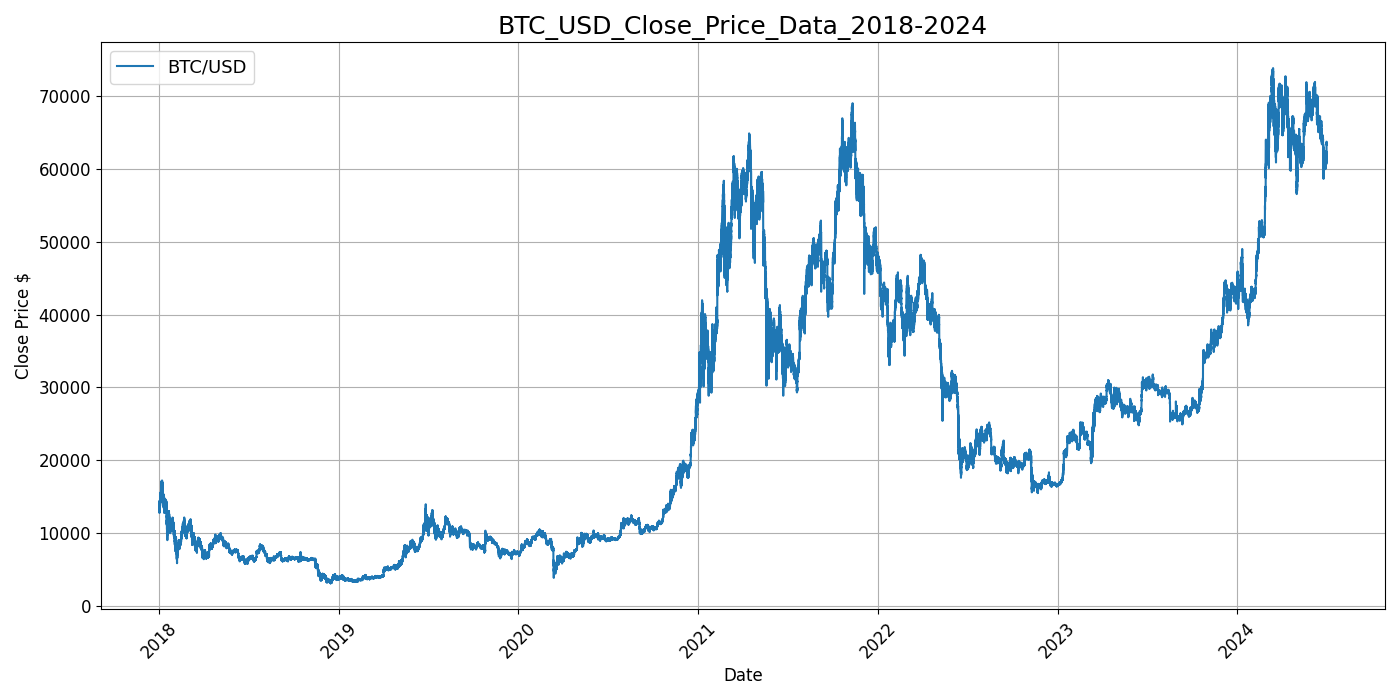
\includegraphics[width=0.8\textwidth]{./figures/BTC_USD_Close_Price_Data_2018-2024.png}
    \caption{Serie Temporal de Precios de Bitcoin}
    \label{fig:bitcoin-prices}
\end{figure}

\subsubsection{Datos del SPY}

El SPY es un ETF que sigue el rendimiento del índice S\&P 500. Los datos del SPY que utilizaremos también incluyen los precios de cierre 
por minuto. A continuación se muestra la serie temporal de precios del SPY:

\begin{figure}[H]
    \centering
    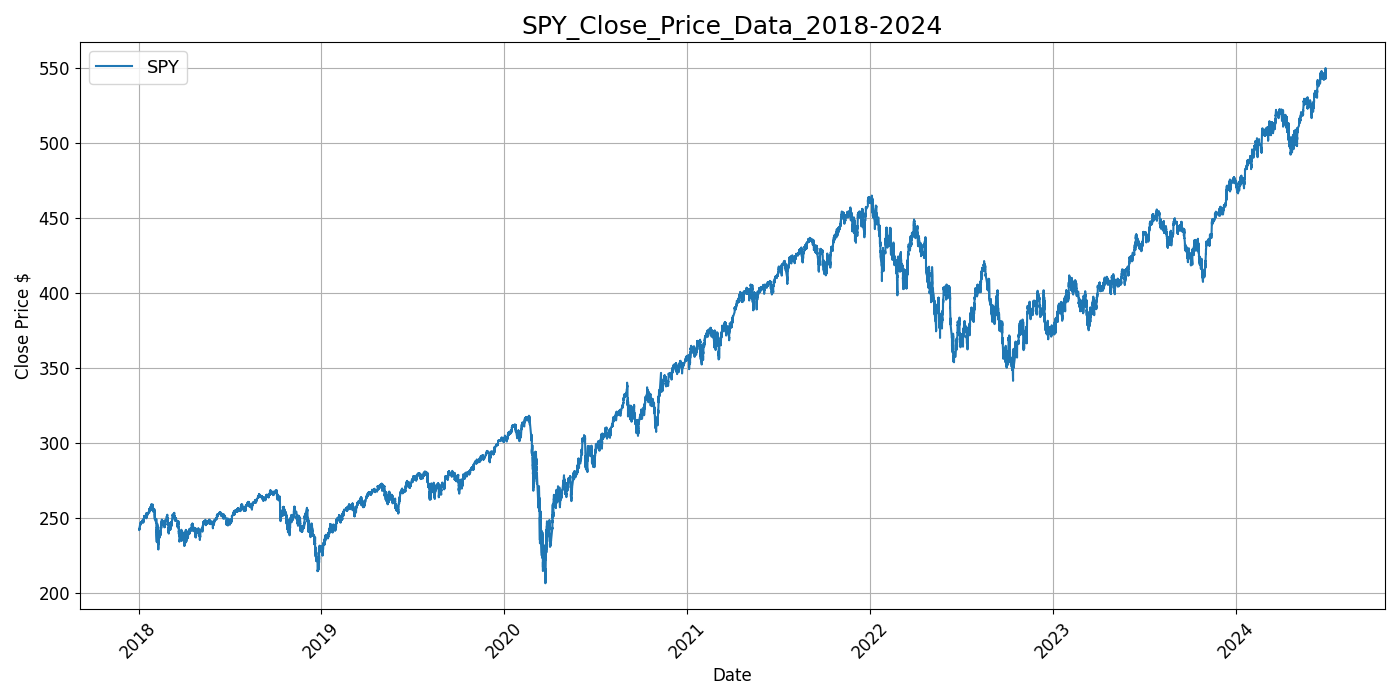
\includegraphics[width=0.8\textwidth]{figures/SPY_Close_Price_Data_2018-2024.png}
    \caption{Serie Temporal de Precios del SPY}
    \label{fig:spy-prices}
\end{figure}

\subsubsection{Propiedades Estadísticas de los Datos}

Para verificar si los datos de Bitcoin y del SPY cumplen con los hechos estilizados, analizaremos sus propiedades estadísticas. 
A continuación se presentan los resultados del análisis:

% \begin{enumerate}
%     \item \textbf{Ausencia de Autocorrelaciones}: Calcularemos la autocorrelación de los retornos de los precios para ambas series temporales y verificaremos si son insignificantes en frecuencias diarias y superiores.
    
%     \begin{figure}[H]
%         \centering
%         \includegraphics[width=0.8\textwidth]{autocorrelation_bitcoin.png}
%         \caption{Autocorrelación de los Retornos de Bitcoin}
%         \label{fig:autocorrelation-bitcoin}
%     \end{figure}
    
%     \begin{figure}[H]
%         \centering
%         \includegraphics[width=0.8\textwidth]{autocorrelation_spy.png}
%         \caption{Autocorrelación de los Retornos del SPY}
%         \label{fig:autocorrelation-spy}
%     \end{figure}
    
%     \item \textbf{Colas Pesadas}: Analizaremos la distribución de los retornos y verificaremos la presencia de colas pesadas comparando con una distribución normal.
    
%     \begin{figure}[H]
%         \centering
%         \includegraphics[width=0.8\textwidth]{histogram_bitcoin.png}
%         \caption{Histograma de los Retornos de Bitcoin}
%         \label{fig:histogram-bitcoin}
%     \end{figure}
    
%     \begin{figure}[H]
%         \centering
%         \includegraphics[width=0.8\textwidth]{histogram_spy.png}
%         \caption{Histograma de los Retornos del SPY}
%         \label{fig:histogram-spy}
%     \end{figure}
    
%     \item \textbf{Asimetría de Ganancias/Pérdidas}: Evaluaremos la asimetría en los movimientos extremos de los precios, identificando si las caídas bruscas son más comunes que los incrementos bruscos.
    
%     \item \textbf{Gaussianidad Agregada}: Verificaremos cómo la distribución de los retornos se aproxima a una distribución normal al aumentar la escala temporal de los retornos.
    
%     \item \textbf{Intermitencia}: Analizaremos la variabilidad de los retornos en diferentes escalas temporales para identificar periodos de alta y baja volatilidad.
    
%     \item \textbf{Agrupamiento de Volatilidad}: Evaluaremos la presencia de clústeres de alta y baja volatilidad en las series temporales de retornos.
    
%     \begin{figure}[H]
%         \centering
%         \includegraphics[width=0.8\textwidth]{volatility_clustering_bitcoin.png}
%         \caption{Agrupamiento de Volatilidad en los Retornos de Bitcoin}
%         \label{fig:volatility-clustering-bitcoin}
%     \end{figure}
    
%     \begin{figure}[H]
%         \centering
%         \includegraphics[width=0.8\textwidth]{volatility_clustering_spy.png}
%         \caption{Agrupamiento de Volatilidad en los Retornos del SPY}
%         \label{fig:volatility-clustering-spy}
%     \end{figure}
    
% \end{enumerate}

Este análisis permitirá verificar si los datos de Bitcoin y del SPY cumplen con los hechos estilizados 
descritos por Cont (2001) \cite{Cont2001}, proporcionando una base sólida para el modelado y la estrategia 
de trading propuesta en este trabajo.

\chapter{Imbalance bars}

\section{Barras Basadas en Información}

En la industria financiera, es común el uso de barras de tiempo para transformar 
series de observaciones que llegan a intervalos irregulares en series homogéneas 
derivadas de un muestreo regular. Las barras de tiempo, obtenidas al muestrear 
información en intervalos de tiempo fijos (por ejemplo, cada minuto), suelen incluir 
datos como la marca temporal, el precio de apertura, el precio de cierre, el precio 
más alto, el más bajo, y el volumen negociado. Estos datos se conocen como datos \textit{ohclv}.

Aunque las barras de tiempo son populares tanto entre los profesionales como entre los académicos, 
el libro de Marcos López de Prado introduce las limitaciones que presentan este tipo de datos:

\begin{itemize}
    \item Los mercados no procesan información a intervalos de tiempo constantes. Por ejemplo, la 
    actividad es significativamente mayor en las horas inmediatamente posteriores a la apertura, 
    en comparación con periodos de menor actividad, como el mediodía.
    \item Las barras de tiempo tienden a sobre-representar la actividad durante periodos tranquilos 
    y sub-representar durante momentos de alta actividad, lo que distorsiona la representatividad de los datos.
    \item Las series temporales basadas en tiempo suelen exhibir propiedades estadísticas deficientes, 
    como correlación serial, heteroscedasticidad y no-normalidad de los retornos, lo que complica el 
    modelado y análisis de los datos.
\end{itemize}

Formar barras basadas en la información de mercado, en lugar de intervalos de tiempo fijos, 
es una alternativa que mejora la representatividad de los datos y las propiedades estadísticas 
de las series temporales generadas. 

Este tipo de barras basadas en información ajustan dinámicamente el tamaño de las barras
en respuesta a la llegada de nueva información, lo que permite una representación
más precisa de las condiciones de mercado.Este enfoque es útil para identificar y reaccionar 
ante la presencia de traders
informados, quienes pueden provocar desequilibrios en los precios.

\subsection{Barras de Desequilibrio}

Las barras de desequilibrio son un tipo de barra basada en información que ajusta el muestreo 
según la actividad del mercado en lugar de hacerlo a intervalos de tiempo fijos. Este enfoque 
permite capturar de manera más efectiva los momentos en que se produce nueva información relevante, 
mejorando así la capacidad de respuesta ante los cambios del mercado.

\subsubsection{La Regla del Tick}

En el ámbito de la microestructura del mercado, es esencial comprender cómo se generan y clasifican las operaciones. En un 
libro de órdenes de subasta doble, se registran cotizaciones para vender (ofertas) y comprar (demandas) un valor a diferentes 
niveles de precios. Las operaciones ocurren cuando un comprador coincide con una oferta o un vendedor con una demanda. La regla 
del tick es una herramienta que permite identificar el lado agresor de cada operación. Esta regla clasifica una transacción 
como iniciada por el comprador si el precio sube (\(\Delta p_t > 0\)) o por el vendedor si el precio baja (\(\Delta p_t < 0\)). 
Si el precio se mantiene igual (\(\Delta p_t = 0\)), la clasificación se mantiene según el último tick registrado:

\begin{equation}
b_t =
\begin{cases}
1 & \text{si} \ \Delta p_t > 0 \\
-1 & \text{si} \ \Delta p_t < 0 \\
b_{t-1} & \text{si} \ \Delta p_t = 0
\end{cases}
\end{equation}

donde \(p_t\) es el precio de la operación indexado por \(t = 1,\ldots,T\) y \(b_0\) se establece arbitrariamente en 1. 
La regla del tick, a pesar de su simplicidad, ha demostrado ser efectiva en la clasificación de transacciones, con una 
alta precisión documentada en varios estudios (Aitken y Frino, 1996).

\subsubsection{Tipos de Barras de Desequilibrio}

\paragraph{Barras de Desequilibrio de Tick (TIB)}

Las barras de desequilibrio de tick se basan en la idea de que el desequilibrio en los ticks puede revelar información 
importante. Se consideran secuencias de ticks donde cada tick tiene un precio \(p_t\) y un volumen \(v_t\). La regla del tick 
se utiliza para generar una secuencia \(\{b_t\}\) que clasifica cada tick como compra o venta. El desequilibrio de tick en un 
intervalo se define como la suma de los ticks clasificados:

\begin{equation}
\theta_T = \sum_{t=1}^{T} b_t
\end{equation}

Para determinar cuándo muestrear una nueva barra, se calcula el desequilibrio esperado \(\theta_T\) al inicio de la barra. 
Este se estima como:

\begin{equation}
E_0[\theta_T] = E_0[T](2P[b_t = 1] - 1)
\end{equation}

donde \(E_0[T]\) es el tamaño esperado de la barra, y \(P[b_t = 1]\) y \(P[b_t = -1]\) son las probabilidades de que un tick 
se clasifique como compra o venta, respectivamente. Una TIB se genera cuando el desequilibrio acumulado excede un umbral basado 
en estas expectativas:

\begin{equation}
T^* = \arg \min_T \left\{  | \theta_T | \geq E_0[\theta_T] |2P[b_t = 1] - 1 | \right\}
\end{equation}

Este tipo de barras se utiliza principalmente en datos de transacciones, ya que ofrecen una visión detallada de cada tick 
en el mercado.

\paragraph{Barras de Desequilibrio de Volumen y Dólares (VIB y DIB)}

Las barras de desequilibrio de volumen y de dólares extienden el concepto de las TIB al considerar el volumen 
y el valor en dólares de las transacciones, respectivamente. El objetivo es identificar desequilibrios en el volumen de 
transacciones o el valor monetario que puedan indicar la presencia de información nueva y relevante.

El desequilibrio en un intervalo se define como:

\begin{equation}
\theta_T = \sum_{t=1}^{T} b_t v_t
\end{equation}

donde \(v_t\) representa el volumen negociado o la cantidad en dólares intercambiado. El valor esperado de este desequilibrio 
se calcula como:

\begin{equation}
E_0[\theta_T] = E_0[T](v_+ - v_-) = E_0[T](2v_+ - E_0[v_t])
\end{equation}

Aquí, \(v_+\) y \(v_-\) representan la contribución esperada del volumen de las compras y ventas, respectivamente. En la 
práctica, \(E_0[T]\) y \(2v_+ - E_0[v_t]\) se estiman usando promedios móviles ponderados exponencialmente. Una VIB o DIB 
se define como un subconjunto \(T^*\) contiguo de ticks tal que:

\begin{equation}
T^* = \arg \min_{T} \{|\theta_T| \geq E_0[T]|2v_+ - E_0[v_t]| \}
\end{equation}

Cuando el desequilibrio \(\theta_T\) excede las expectativas, las barras se generan con mayor frecuencia, reflejando la 
presencia de traders informados y ajustando dinámicamente el tamaño de las barras según la información disponible.

\subsection{Adaptación de la Metodología con Datos de Minuto}

La metodología presentada en el libro de Marcos López de Prado está diseñada originalmente para trabajar con datos de tick, 
los cuales proporcionan un registro extremadamente detallado de cada transacción individual en el mercado. Los datos de tick 
incluyen información específica sobre el precio, el volumen y el tiempo exacto en el que se realiza cada operación, lo que 
permite una representación precisa y granular de la actividad del mercado. Este nivel de detalle permite capturar la dinámica 
completa del mercado, especialmente cuando se busca identificar patrones como desequilibrios en la oferta y la demanda que 
pueden indicar la presencia de traders informados.

Los datos de tick son valiosos porque reflejan cada cambio en el mercado en tiempo real, permitiendo un análisis fino de la 
microestructura del mercado. Sin embargo, obtener estos datos puede ser complicado y costoso, debido a la gran cantidad de 
información que se genera y la necesidad de acceder a servicios de datos financieros especializados.

Dada la dificultad para obtener datos de tick, en este estudio se opta por utilizar datos de minuto, debido a su accesibilidad 
y facilidad de manejo. Los datos de minuto agregan todas las transacciones que ocurren dentro de un minuto, ofreciendo una 
visión resumida de la actividad del mercado durante ese intervalo de tiempo. Aunque esta aproximación sacrifica cierta 
granularidad, sigue siendo adecuada para el análisis de tendencias y patrones en el mercado.

Se han obtenido series temporales de datos de minuto para Bitcoin y el ETF SPY a través de las APIs de Alpha Vantage y 
Financial Modelling Prep, de forma gratuita. Estos datos fueron procesados para incluir únicamente las transacciones 
realizadas dentro del horario de mercado: 24 horas al día en el caso de Bitcoin, y el horario estándar del mercado para 
el ETF SPY. Además, se han interpolado las muestras faltantes propagando hacia adelante el valor del minuto anterior, 
asegurando así la continuidad de la serie temporal.

Para implementar la metodología de barras de desequilibrio con estos datos, se utilizará el precio de cierre de cada minuto 
como proxy del precio de transacción. Este enfoque simplifica la aplicación de la metodología, permitiendo su adaptación a 
los datos disponibles, mientras se mantiene la integridad del análisis basado en la llegada de nueva información relevante 
al mercado.

\subsubsection{Implementación}
La implementación de las barras de desequilibrio requiere una cuidadosa consideración de los parámetros iniciales, 
ya que estos son fundamentales para el cálculo del primer valor esperado de ticks en una barra (\(E_0[T]\)). Al inicio 
del proceso, no se dispone de barras previas que puedan proporcionar una estimación de \(E_0[T]\), por lo que es necesario 
hacer una suposición inicial. A medida que se generan más barras, \(E_0[T]\) se ajusta dinámicamente utilizando un promedio móvil exponencialmente 
ponderado (EWMA) basado en los valores de \(T\) de las barras anteriores.

Los gráficos presentados en las Figuras \ref{fig:barrido-spy} y \ref{fig:barrido-btc} muestran el número de barras 
generadas para el ETF SPY y el Bitcoin (BTC) al aplicar la metodología de barras de desequilibrio, utilizando como 
parámetros iniciales \texttt{ewma\_window}, \texttt{T\_init} y \texttt{imbalance\_init}. Los datos del SPY cuentan 
con 662,353 muestras iniciales, mientras que los del BTC cuentan con 3,417,119. El parámetro \texttt{imbalance\_init} 
se inicializa con la media histórica del volumen, mientras que \texttt{ewma\_window} y \texttt{T\_init} se han ajustado 
a través de un barrido de valores. 

Los gráficos reflejan cómo la variación de estos parámetros afecta la frecuencia de barras 
generadas. Específicamente, con parámetros iniciales bajos, la cantidad de desequilibrio necesario para generar una 
nueva barra aumenta de manera explosiva, lo que lleva a una rápida reducción en la frecuencia de barras generadas. 
Por otro lado, con parámetros iniciales altos, el desequilibrio necesario para el sampleo es demasiado bajo, 
resultando en un número de barras generadas que es prácticamente idéntico al número de barras iniciales. 


\begin{figure}[H]
    \centering
    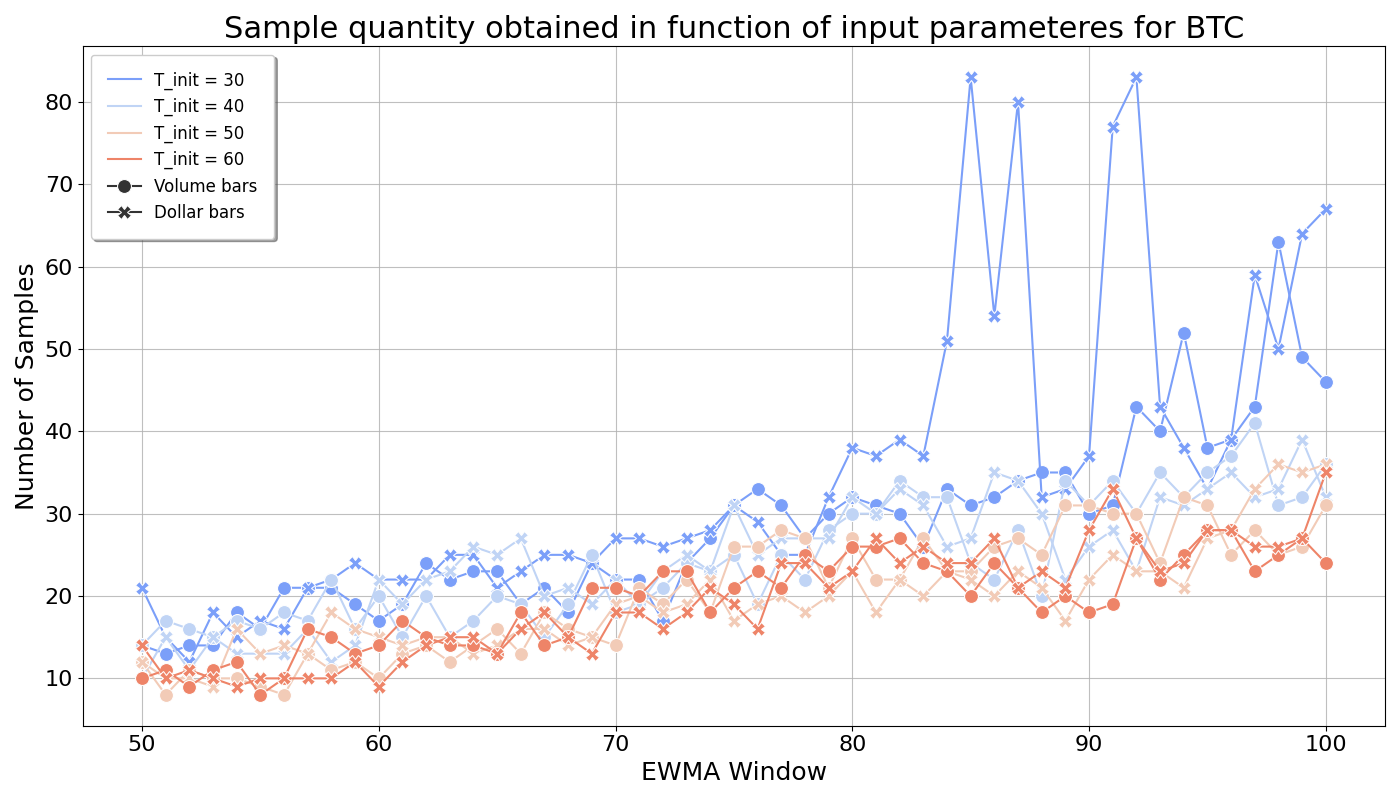
\includegraphics[width=0.9\textwidth]{./figures/barrido_parametros_imbalance_btc.png}
    \caption{Número de barras obtenido en datos de BTC}
    \label{fig:barrido-btc}
\end{figure}

\begin{figure}[H]
    \centering
    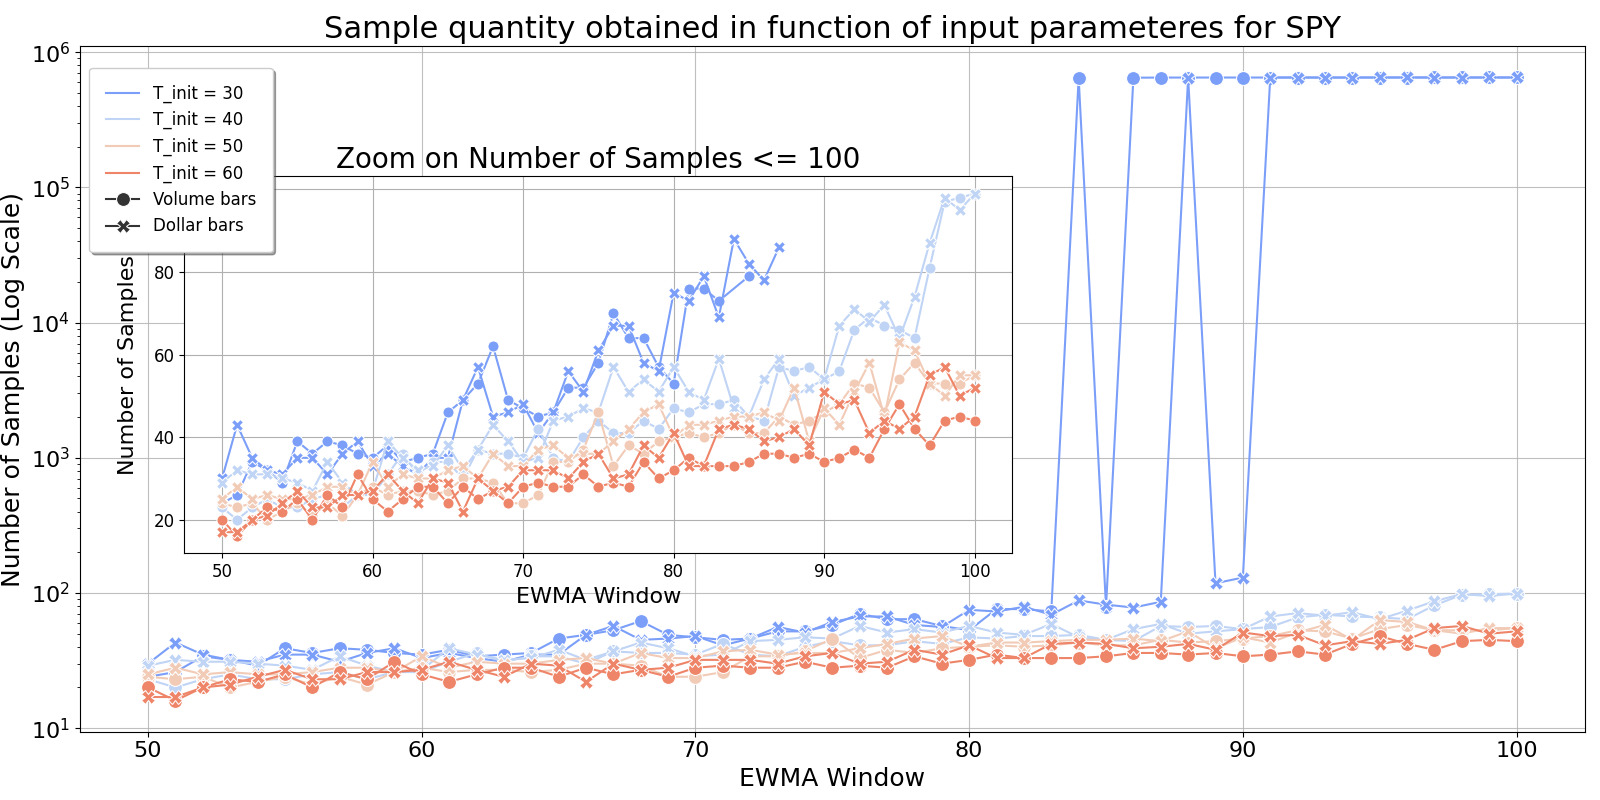
\includegraphics[width=0.9\textwidth]{./figures/barrido_parametros_imbalance_spy.png}
    \caption{Número de barras obtenido en datos del SPY}
    \label{fig:barrido-spy}
\end{figure}

Este comportamiento muestra un problema crítico en la implementación: la dinámica de generación de barras tiende a explotar, 
tal y como se muestra en la figura \ref{fig:explo-spy}. A medida que se van generando nuevas barras, el humbral de desequilibrio,
es decir, el producto de la multiplicacion del tamaño esperado de la barra por el desequilibrio esperado, provoca que el humbral de
desequilibrio sea cada vez mayor.

\begin{figure}[H]
    \centering
    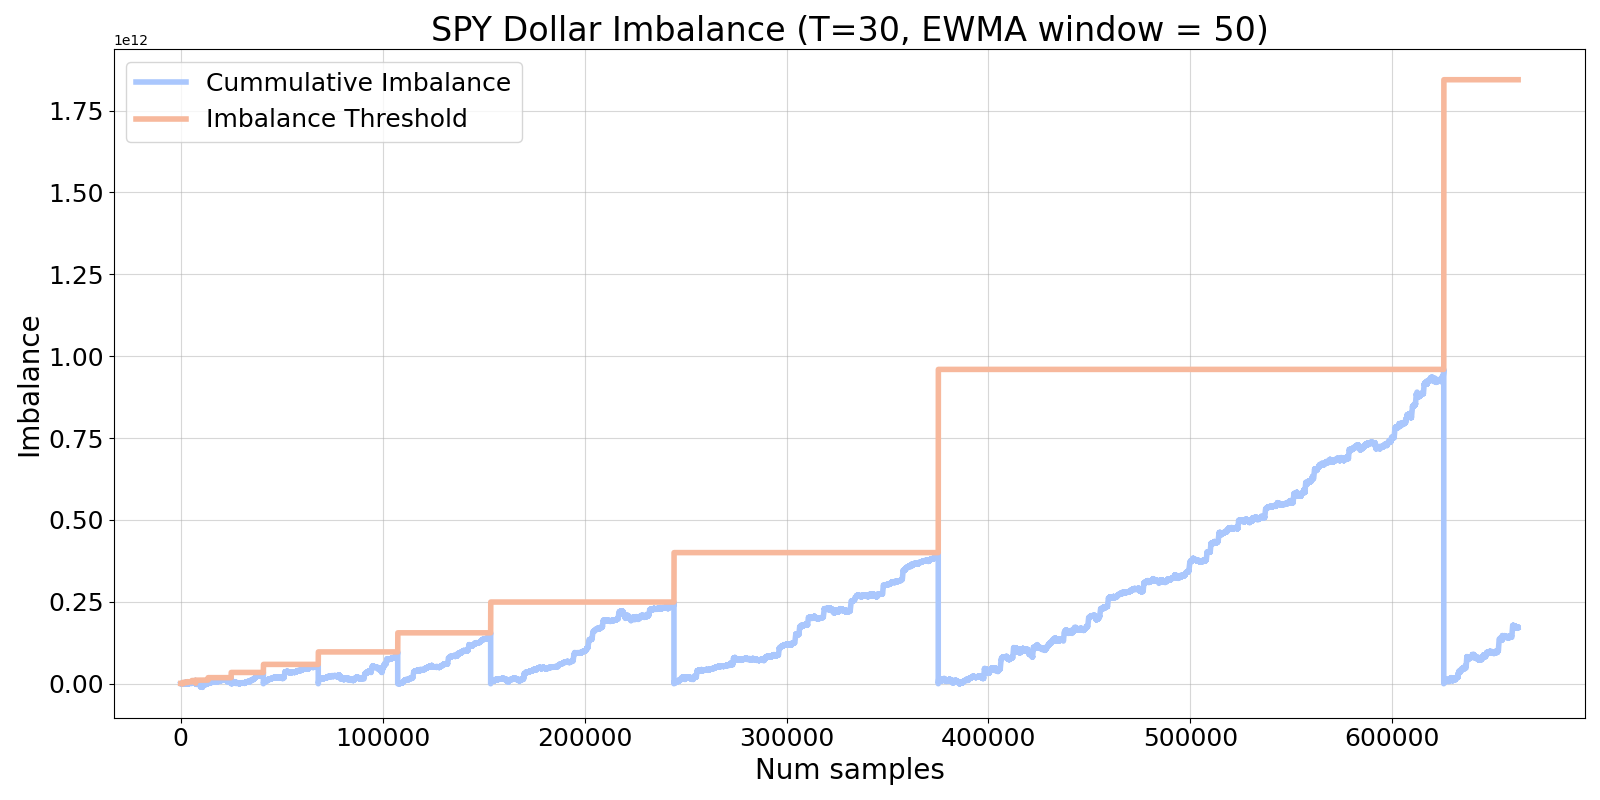
\includegraphics[width=0.9\textwidth]{./figures/spy_volume_explo.png}
    \caption{Explosión del umbral de desequilibrio en SPY}
    \label{fig:explo-spy}
\end{figure}

Para hacer frente a este problema, algunos investigadores han propuesto modificaciones 
a la implementación sugerida, tales como establecer un límite máximo al número esperado 
de ticks por barra o seleccionar directamente un umbral fijo de desequilibrio \cite{quant_finance_stack_exchange}. 

\subsection{Resultados}
Para este trabajo, se ha optado por aplicar la metodología con umbrales de desequilibrio fijos, definidos experimentalmente.
Para cada activo y tipo de desequilibrio se ha seleccionado un umbral distinto, tal y como se muestra en la tabla \ref{tab:umbrales}.

\begin{table}[H]
    \centering
    \caption{Umbrales utilizados y numero de muestras obtenido}
    \begin{tabularx}{\textwidth}{|>{\centering\arraybackslash}X|>{\centering\arraybackslash}X|>{\centering\arraybackslash}X|>{\centering\arraybackslash}X|>{\centering\arraybackslash}X|>{\centering\arraybackslash}X|}
        \hline
        \textbf{Activo} & \textbf{Des- equilibrio} & \textbf{Umbral} & \textbf{Muestras iniciales} & \textbf{Muestras finales} & \textbf{Reducción (\%)} \\ \hline
        SPY & Volumen & $6 \times 10^{5}$ & 662,353 & 55,430 & 91.63\% \\ \hline
        SPY & Dólar & $1.5 \times 10^{8}$ & 662,353 & 85,228 & 87.13\% \\ \hline
        BTC & Volumen & $5 \times 10^{6}$ & 3,417,119 & 110,772 & 96.76\% \\ \hline
        BTC & Dólar & $1.5 \times 10^{10}$ & 3,417,119 & 1,003,756 & 70.63\% \\ \hline
    \end{tabularx}
    \label{tab:umbrales}
\end{table}

Los umbrales de desequilibrio se han definido con el fin de obtener una disminución significativa del numero de muestras de cada activo. Las 
disminuciones en la cantidad de datos van desde el 70\% para el desequilibrio de dolares de bitcoin, hasta el 96\% para el desequilibrio en volumen del
mismo activo.

En la Figura \ref{fig:btc-vol-imb-comp} se muestra una comparativa de los datos de precio originales de bitcoin y 
los de desequilibrio de volumen durante durante un segmento perteneciente al período de alta volatilidad ocasionada 
por la pandemia de COVID-19. Se puede observar cómo, para el mismo período de tiempo, las barras generadas mediante la metodología de desequilibrio 
son menos numerosas que las barras de minuto originales. 

Este fenómeno se debe a la agregación dinámica de los datos basada en la llegada de nueva información relevante, lo que permite una representación más frecuente
durante periodos de alta actividad de mercado.

\begin{figure}[H]
    \centering
    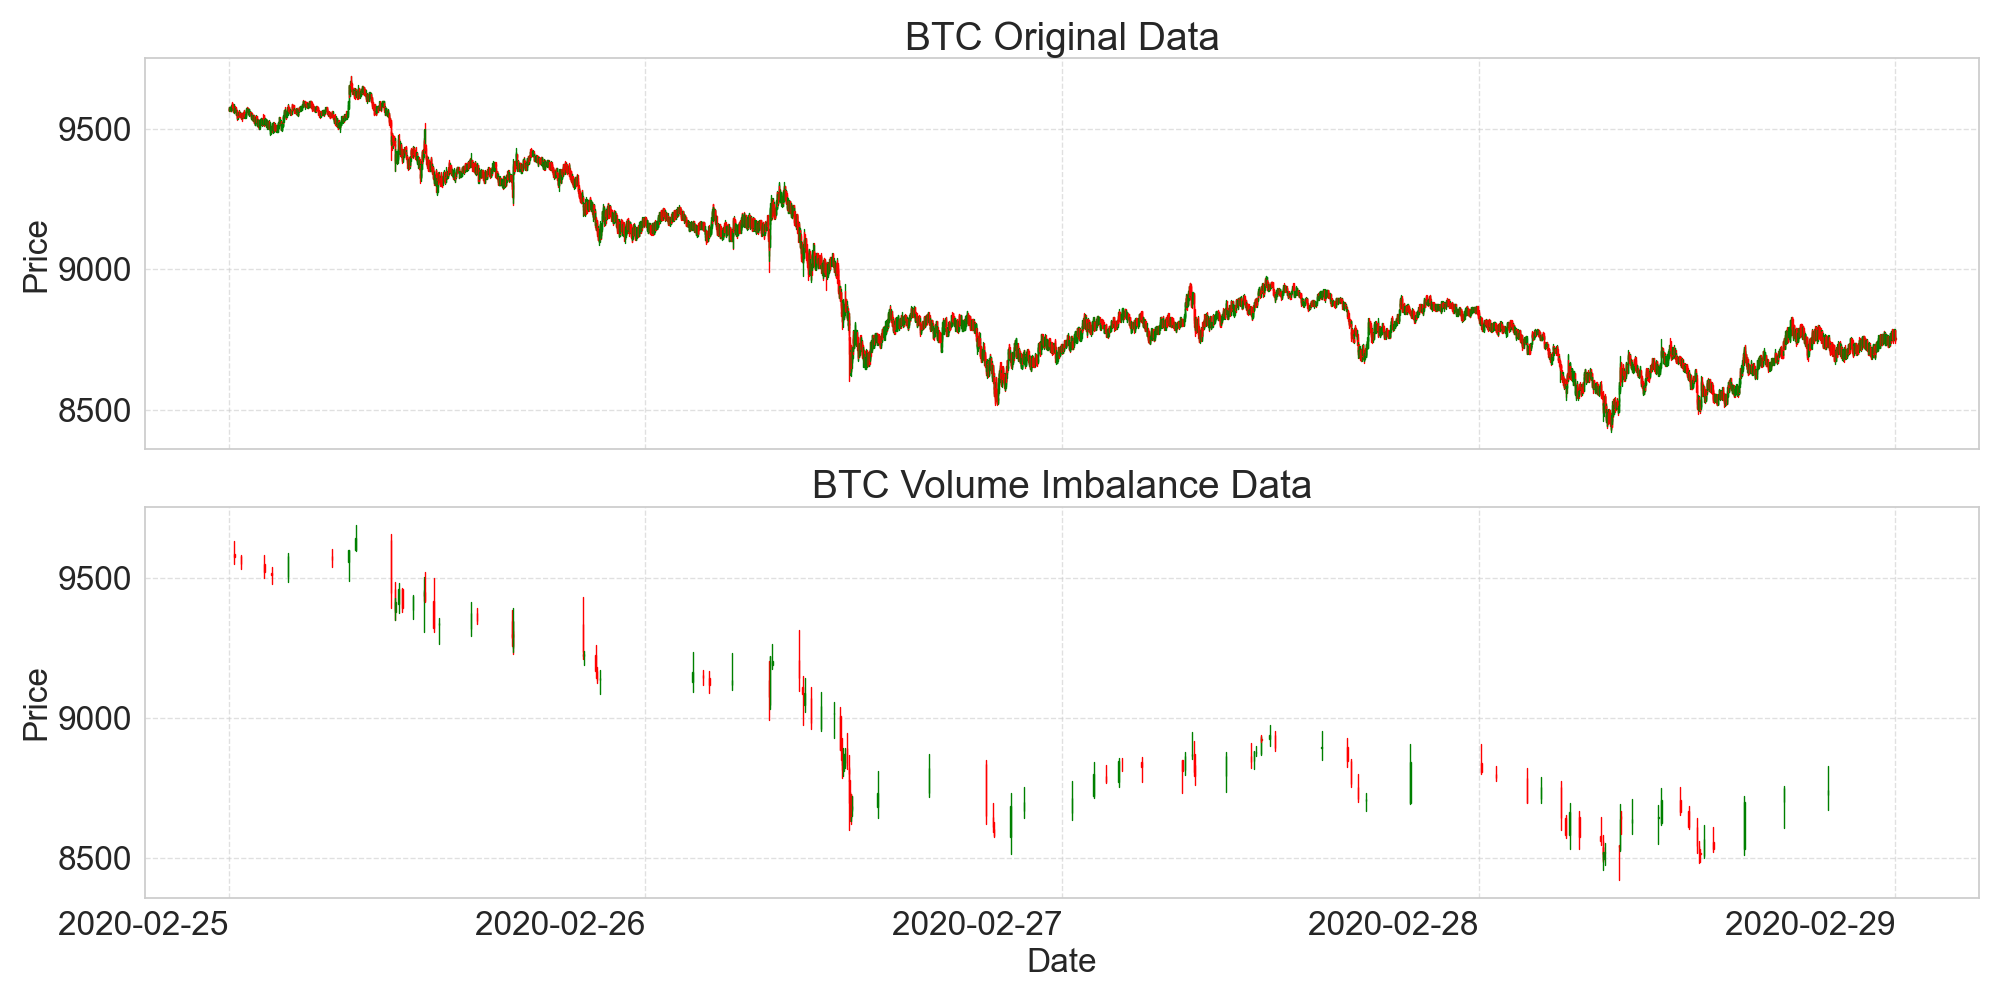
\includegraphics[width=0.9\textwidth]{./figures/btc_original_volume_imabalance_comp.png}
    \caption{Datos BTC originales y de Desequilibrio de Volumen}
    \label{fig:btc-vol-imb-comp}
\end{figure}

El artículo de Easley, López de Prado y O'Hara titulado "The Volume Clock: Insights into the High Frequency 
Paradigm" \cite{easley2012volume} expone que el uso de un marco temporal basado en volumen, en lugar de un 
marco cronológico tradicional, ofrece ventajas estadísticas significativas. Entre ellas, se destaca que 
este enfoque permite una reducción de los efectos estacionales intra-sesión y contribuye a una recuperación 
parcial de la normalidad en la distribución de los retornos financieros. Para evaluar esta afirmación, se 
ha aplicado la metodología de desequilibrio propuesta por los autores a los activos SPY y BTC, generando 
series temporales basadas en volumen y dinero.

Con el fin de verificar la normalidad de los retornos obtenidos mediante esta metodología, se han realizado 
pruebas estadísticas de normalidad, incluyendo los tests de Kolmogorov-Smirnov, Anderson-Darling y Jarque-Bera, 
cuyos resultados se resumen en la Tabla \ref{tab:normality_results}. Los resultados muestran que las series 
temporales originales de ambos activos presentan una desviación significativa de la normalidad, con valores 
extremadamente elevados de curtosis y asimetría, especialmente en el caso del SPY. 

Tras la aplicación de barras dinámicas basadas en volumen y dolares, se observa una reducción considerable 
en la curtosis y asimetría de los retornos. En particular, las barras basadas en volumen han demostrado 
ser más efectivas para aproximar la distribución de retornos a una forma más cercana a la normalidad. 
Estos resultados confirman en gran medida las hipótesis expuestas en el trabajo de Easley, López de Prado y O'Hara, 
evidenciando que el uso de un marco temporal basado en volumen contribuye a mejorar las propiedades 
estadísticas de las series temporales, aunque persisten algunas desviaciones de la normalidad, 
especialmente en los datos de BTC.


\begin{table}[H]
    \centering
    \caption{Resultados de pruebas estadísticas de normalidad para SPY y BTC}
    \begin{tabularx}{\textwidth}{|m{1cm}|m{1.35cm}|>{\centering\arraybackslash}X|>{\centering\arraybackslash}X|>{\centering\arraybackslash}X|>{\centering\arraybackslash}X|>{\centering\arraybackslash}X|>{\centering\arraybackslash}X|}
        \hline
        \textbf{Asset} & 
        \textbf{Series} & 
        \textbf{K-S Test \newline p-value} & 
        \textbf{Anderson-Darling \newline Statistic} & 
        \textbf{Jarque-Bera \newline p-value} & 
        \textbf{Skewness} & \textbf{Kurtosis} \\ \hline
        SPY & Original & 0.0 & 46037.02 & 0.0 & -11.83 & 2981.95 \\ \hline
        SPY & Volume & 0.0 & 1553.58 & 0.0 & -3.46 & 249.67 \\ \hline
        SPY & Dollar & 0.0 & 2947.14 & 0.0 & -4.24 & 383.73 \\ \hline
        BTC & Original & 0.0 & 646407.27 & 0.0 & 0.012 & 44.68 \\ \hline
        BTC & Volume & 0.0 & 3131.35 & 0.0 & -0.026 & 26.13 \\ \hline
        BTC & Dollar & 0.0 & 97255.28 & 0.0 & 0.070& 139.58 \\ \hline
    \end{tabularx}
    \label{tab:normality_results}
\end{table}

Además de las pruebas estadísticas, se han generado cuatro representaciones visuales que comparan 
las distribuciones de retornos de los activos SPY y BTC antes y después de aplicar la metodología 
basada en volumen y dinero. La Figura \ref{fig:histogram_comparison} muestra una comparativa de 
los histogramas de los retornos para el SPY y el BTC, donde se observa cómo la transformación 
mediante barras dinámicas logra atenuar la asimetría y la curtosis extrema presentes en las series 
temporales originales. 

Por otro lado, en la Figura \ref{fig:qqplot_comparison}, se presentan los QQ-plots correspondientes, 
que permiten evaluar visualmente el grado de ajuste de los retornos a una distribución normal. 
Los QQ-plots evidencian una mejora en la alineación con la diagonal en las series ajustadas, 
especialmente para el SPY, lo que sugiere una aproximación más cercana a la normalidad tras la 
aplicación de la metodología propuesta. 

\begin{figure}[H]
    \centering
    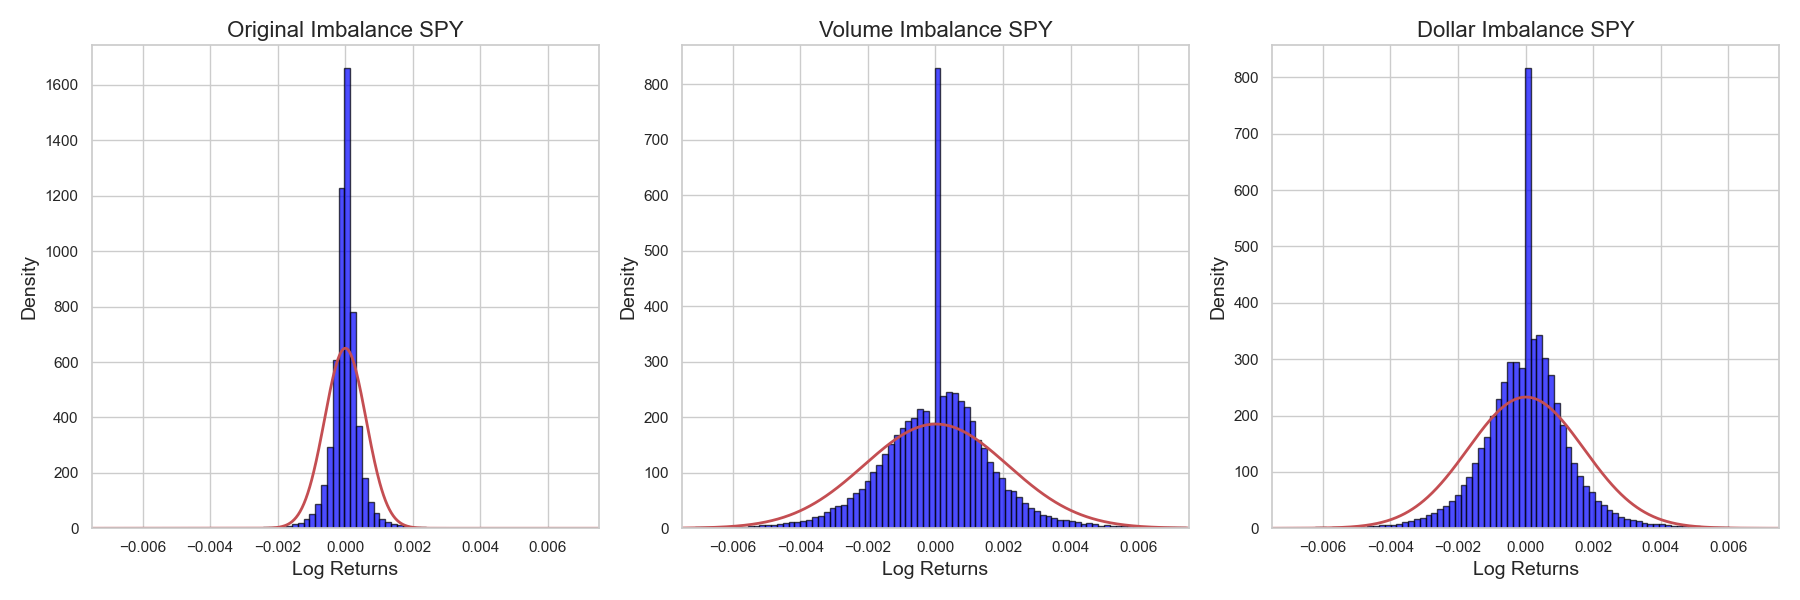
\includegraphics[width=0.8\textwidth]{figures/SPY_histogram_comparation.png}
    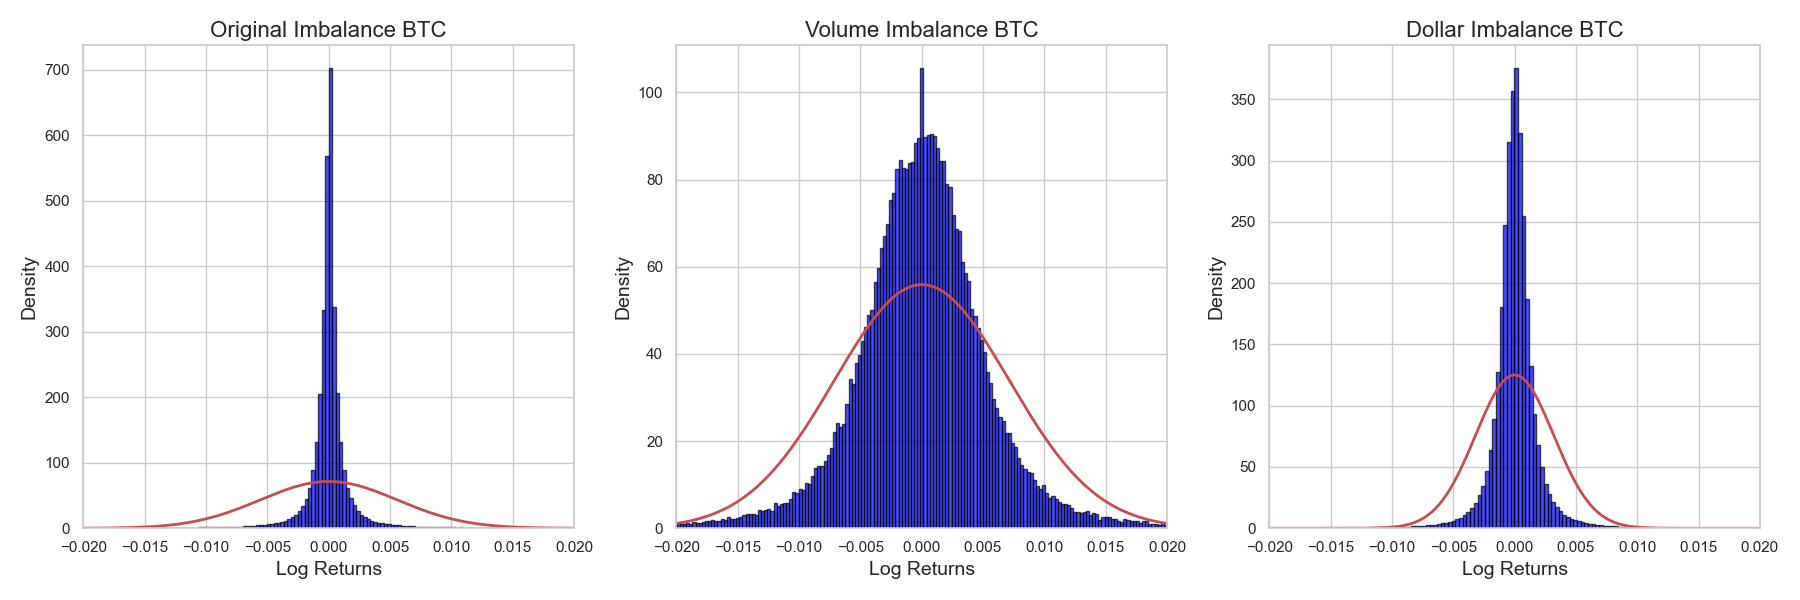
\includegraphics[width=0.8\textwidth]{figures/BTC_histogram_comparation.png}
    \caption{Comparativa de histogramas de los retornos del SPY (arriba) y BTC (abajo)}
    \label{fig:histogram_comparison}
\end{figure}

\begin{figure}[H]
    \centering
    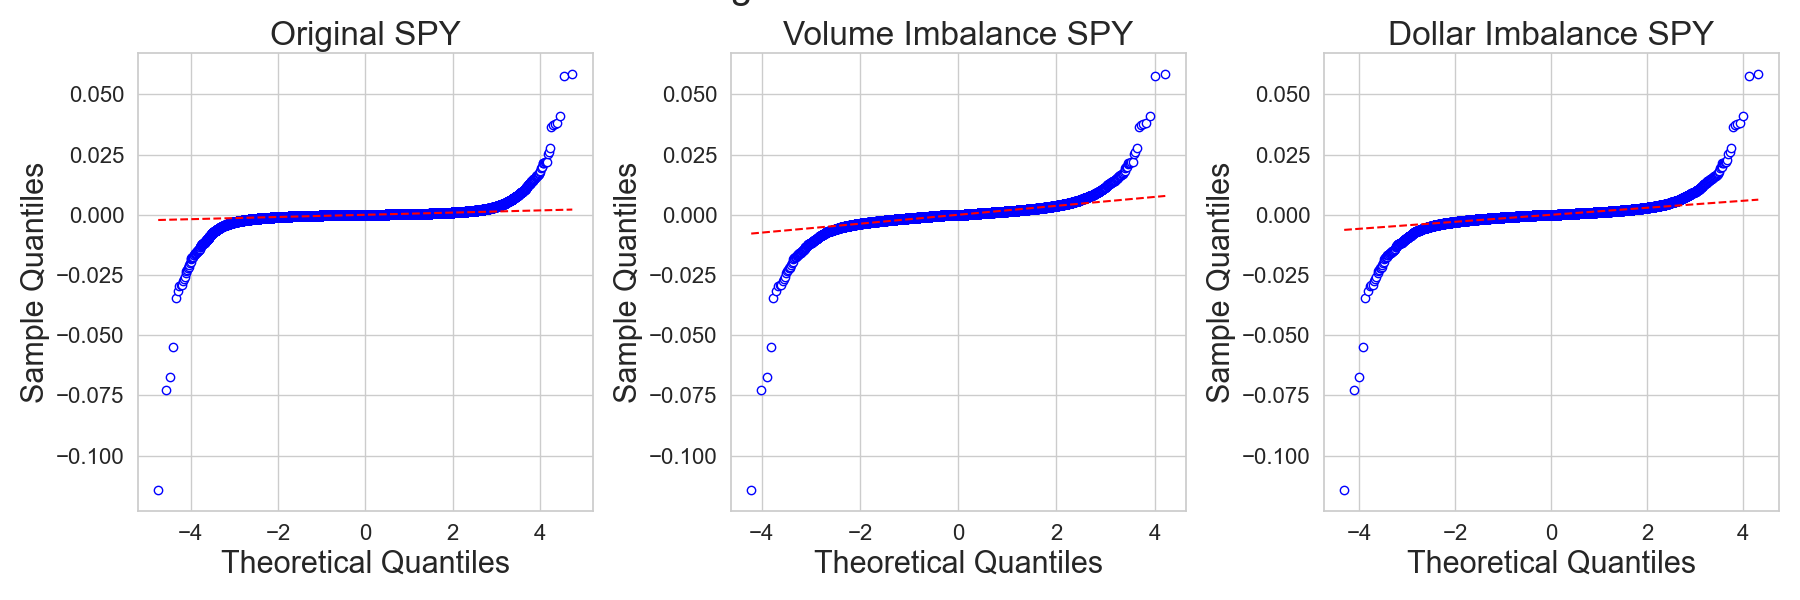
\includegraphics[width=0.8\textwidth]{figures/SPY_qq_comparison.png}
    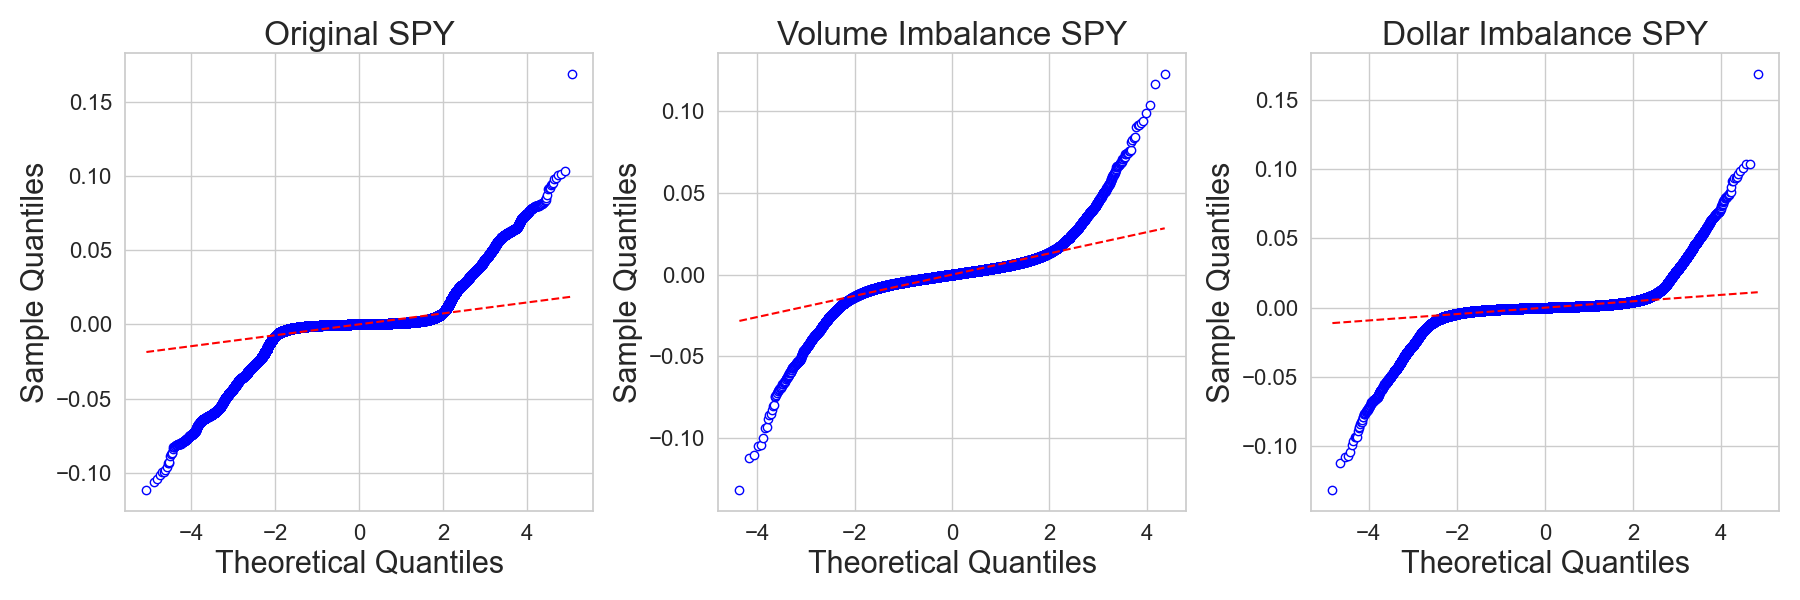
\includegraphics[width=0.8\textwidth]{figures/BTC_qq_comparison.png}
    \caption{Comparativa de QQ-plots de los retornos del SPY (arriba) y BTC (abajo)}
    \label{fig:qqplot_comparison}
\end{figure}

\chapter{Deep Reinforcement Learning}

\section{Introducción al Aprendizaje por Refuerzo (Reinforcement Learning)}

\subsection{Definición y Contexto General}

El \textit{Aprendizaje por Refuerzo} (Reinforcement Learning, RL) es una rama dentro de la inteligencia 
artificial que se centra en cómo un agente aprende a tomar decisiones secuenciales optimizadas mediante 
la interacción con un entorno dinámico. A diferencia de otros tipos de aprendizaje como el 
\textit{aprendizaje supervisado}, donde el modelo aprende patrones extraídos de ejemplos previamente 
etiquetados, o el \textit{aprendizaje no supervisado}, donde el modelo busca patrones en datos sin 
etiquetas, un agente de RL basa su aprendizaje en la retroalimentación recibida por el entorno en 
forma de recompensas o penalizaciones por las acciones que toma.

En un entorno de RL, se define un \textit{Proceso de Decisión de Markov} (MDP, por sus siglas en inglés), 
el cual describe el problema de decisión. Un MDP se representa por un conjunto de estados \(S\), 
un conjunto de acciones \(A\), una función de transición de estados \(P(s'|s, a)\), y una función de 
recompensa \(R(s, a)\). El objetivo del agente es aprender una política \(\pi(a|s)\) que maximice la 
recompensa acumulada a lo largo del tiempo. Este marco es ampliamente aplicable en situaciones donde 
las decisiones se toman en una serie de pasos, lo que incluye problemas de control robótico, juegos, 
y \textit{trading} financiero.

En el contexto particular del trading financiero, debido a la naturaleza secuencial y dinámica de 
los mercados, los agentes deben tomar decisiones basadas en información incompleta y en constante 
cambio, buscando maximizar una recompensa a largo plazo, como la rentabilidad de una cartera.

\subsection{Componentes Básicos del Aprendizaje por Refuerzo}

El proceso de RL se puede modelar mediante un \textit{Proceso de Decisión de Markov} 
(Markov Decision Process, MDP), que se define por un cuarteto \(\langle S, A, P, R \rangle\):


\begin{itemize}
    \item \textbf{Estados (\(S\))}: Representan todas las posibles situaciones en las que se puede 
    encontrar el agente dentro del entorno.
    \item \textbf{Acciones (\(A\))}: Conjunto de todas las decisiones que el agente puede tomar 
    desde cualquier estado dado.
    \item \textbf{Función de Transición de Estados (\(P\))}: Describe la probabilidad de transitar 
    del estado \(s\) al estado \(s'\) como resultado de realizar una acción \(a\), es decir, \(P(s'|s, a)\).
    \item \textbf{Función de Recompensa (\(R\))}: Proporciona una recompensa \(r\) que el agente 
    recibe al transitar del estado \(s\) al estado \(s'\) al realizar la acción \(a\), es decir, \(R(s, a, s')\).
\end{itemize}

El objetivo del agente en RL es aprender una \textit{política} \(\pi(a|s)\) que maximice la recompensa 
acumulada a lo largo del tiempo. La política puede ser determinista, donde una acción específica es 
seleccionada para cada estado, o estocástica, donde se asigna una distribución de probabilidad a las
acciones en cada estado.

Un concepto fundamental en RL es la \textit{función de valor}, que mide cuán favorable es un estado 
o una acción en términos de la recompensa esperada:

\begin{itemize}
    \item \textbf{Función de Valor de Estado (\(V^{\pi}(s)\))}: Estima la recompensa total esperada 
    comenzando desde el estado \(s\) y siguiendo la política \(\pi\). Formalmente, se define como:
    \[
    V^{\pi}(s) = \mathbb{E}\left[\sum_{t=0}^{\infty} \gamma^t R(s_t, a_t) \mid s_0 = s, \pi\right]
    \]
    donde \(\gamma \in [0, 1]\) es el factor de descuento que determina la importancia de las 
    recompensas futuras. Esta función refleja el valor a largo plazo de estar en un estado particular 
    bajo una política dada.

    La función de valor del estado, \(V^{\pi}(s)\), trata de cuantificar \textit{cómo de bueno} es 
    estar en un estado \(s\) cuando se sigue una política \(\pi\).

    \item \textbf{Función de Valor de Acción (\(Q^{\pi}(s, a)\))}: Extiende la función de valor del 
    estado para considerar no solo el estado \(s\), sino también la acción \(a\) tomada en ese estado. 
    Esta función estima la recompensa total esperada al tomar la acción \(a\) en el estado \(s\) y 
    seguir la política \(\pi\) posteriormente:
    \[
    Q^{\pi}(s, a) = \mathbb{E}\left[\sum_{t=0}^{\infty} \gamma^t R(s_t, a_t) \mid s_0 = s, a_0 = a, \pi\right]
    \]
    La función de valor de la acción, \(Q^{\pi}(s, a)\), trata de medir \textit{cómo de buena} es una 
    acción \(a\) específica en un estado \(s\) determinado cuando se sigue la política \(\pi\) después.
 
\end{itemize}

En resumen, la función del valor del estado, \(V^{\pi}(s)\), mide cuán bueno es estar en un estado dado 
bajo una política \(\pi\), mientras que \(Q^{\pi}(s, a)\) mide cuán buena es una acción específica en 
ese estado.


\subsubsection{Exploración vs. Explotación}

En el Aprendizaje por Refuerzo, un desafío clave es el equilibrio entre \textit{exploración} y 
\textit{explotación}. Este balance es fundamental para el aprendizaje efectivo del agente:

\begin{itemize}
    \item \textbf{Exploración}: El agente intenta nuevas acciones para descubrir si existen mejores 
    recompensas disponibles. La exploración es crucial cuando el agente no tiene suficiente conocimiento 
    del entorno y necesita recolectar más información.
    \item \textbf{Explotación}: El agente selecciona la mejor acción conocida basada en su 
    política actual para maximizar la recompensa inmediata. La explotación se basa en la información 
    acumulada y tiene como objetivo maximizar la recompensa a corto plazo.
\end{itemize}

El \textit{trade-off} entre exploración y explotación es crucial porque un agente que explora 
demasiado podría no aprovechar las recompensas conocidas, mientras que un agente que explota 
demasiado podría perder oportunidades para descubrir estrategias más efectivas. 

Existen diversas estrategias para manejar este trade-off, como la \textit{política epsilon-greedy}, 
donde con una probabilidad \(\epsilon\), el agente explora una acción al azar, y con 
una probabilidad \(1-\epsilon\), explota la mejor acción conocida. El valor de \(\epsilon\) 
generalmente disminuye a medida que el agente gana más confianza en su política, lo que permite 
una mayor explotación con el tiempo.

\subsection{Métodos Clásicos de Aprendizaje por Refuerzo}

Existen varios algoritmos clásicos de RL que permiten a los agentes aprender políticas óptimas. Los 
algoritmos se clasifican principalmente en dos categorías: \textit{on-policy} y \textit{off-policy}. 
Estos términos se refieren a la relación entre la política que se está evaluando y mejorando y la 
política que se está utilizando para generar las acciones y, por lo tanto, las experiencias (es decir, 
las transiciones estado-acción-recompensa) que se utilizan para actualizar el modelo.

Un algorítmo de tipo \textit{on-policy} es aquel en el que la política que se optimiza es la misma que 
se utiliza para interactuar con el entorno y generar experiencias.Es decir, se evalúa y mejora la misma
política que se sigue durante el proceso de aprendizaje. Mientras que un algorítmo del tipo \textit{off-policy}
es quel en el que la política que se intenta optimizar es diferente de la política utilizada para generar
las experiencias. Esto permite optimizar una política mientras se sigue otra.

Un ejemplo de algoritmos representativos de cada una de estas categorías son los siguientes:


\begin{itemize}
    \item \textbf{Q-learning}: Un algoritmo \textit{off-policy} que aprende la función de valor de 
    acción \(Q(s, a)\) actualizando iterativamente las estimaciones en función de las recompensas recibidas:
    \[
    Q(s_t, a_t) \leftarrow Q(s_t, a_t) + \alpha \left[r_{t+1} + \gamma \max_{a'} Q(s_{t+1}, a') - Q(s_t, a_t)\right]
    \]
    donde \(\alpha\) es la tasa de aprendizaje. Como algoritmo \textit{off-policy}, Q-learning aprende la 
    política óptima independientemente de la política que el agente sigue durante la exploración. 
    Esto significa que la política utilizada para seleccionar acciones (\textit{behavior policy}) 
    puede ser diferente de la política que se está optimizando (\textit{target policy}).

    \item \textbf{SARSA}: Un algoritmo \textit{on-policy} que, a diferencia de Q-learning, sigue la 
    política actual para actualizar la función \(Q(s, a)\). La actualización en SARSA se realiza 
    utilizando la acción que el agente realmente toma, lo que significa que la política utilizada 
    para seleccionar acciones es la misma que se está optimizando:
    \[
    Q(s_t, a_t) \leftarrow Q(s_t, a_t) + \alpha \left[r_{t+1} + \gamma Q(s_{t+1}, a_{t+1}) - Q(s_t, a_t)\right]
    \]
    Como resultado, SARSA tiende a ser más conservador en su aprendizaje, ya que la política sigue 
    siendo consistente entre el aprendizaje y la ejecución.

\end{itemize}

Los algoritmos \textit{on-policy}, como SARSA, tienen la ventaja de ser coherentes con la política 
actual, lo que puede resultar en un aprendizaje más seguro y estable en entornos dinámicos. Sin embargo, 
pueden ser menos eficientes, ya que dependen exclusivamente de las experiencias generadas por la misma 
política que se está optimizando, lo que puede limitar la exploración. Por otro lado, los algoritmos 
off-policy, como Q-Learning, son más flexibles y permiten un aprendizaje más eficiente al poder optimizar 
una política óptima mientras se sigue una política diferente, más exploratoria. Sin embargo, esta 
flexibilidad puede conllevar complejidad adicional y posibles problemas de estabilidad durante el 
proceso de aprendizaje.

Estos métodos son fundamentales para entender cómo los agentes pueden aprender a tomar decisiones 
óptimas en entornos inciertos y son la base sobre la cual se construyen los métodos más avanzados 
como el \textit{Deep Reinforcement Learning} (DRL).


\section{Introducción al Aprendizaje por Refuerzo (Reinforcement Learning)}

\subsection{Definición y Contexto General}

El \textit{Aprendizaje por Refuerzo} (Reinforcement Learning, RL) es una rama de la inteligencia 
artificial que se centra en cómo un agente aprende a tomar decisiones secuenciales optimizadas 
mediante la interacción con un entorno dinámico. A diferencia de otros tipos de aprendizaje, como 
el \textit{aprendizaje supervisado}, donde el modelo aprende patrones extraídos a partir de ejemplos 
previamente etiquetados, o el \textit{aprendizaje no supervisado}, donde el modelo busca patrones 
en datos sin etiquetas, el RL implica un aprendizaje activo donde el agente recibe retroalimentación 
en forma de recompensas o penalizaciones por las acciones que toma. Este proceso permite al 
agente aprender sin ejemplos de comportamiento óptimo, optimizando en su lugar una señal de recompensa.

\begin{figure}[H]
    \centering
    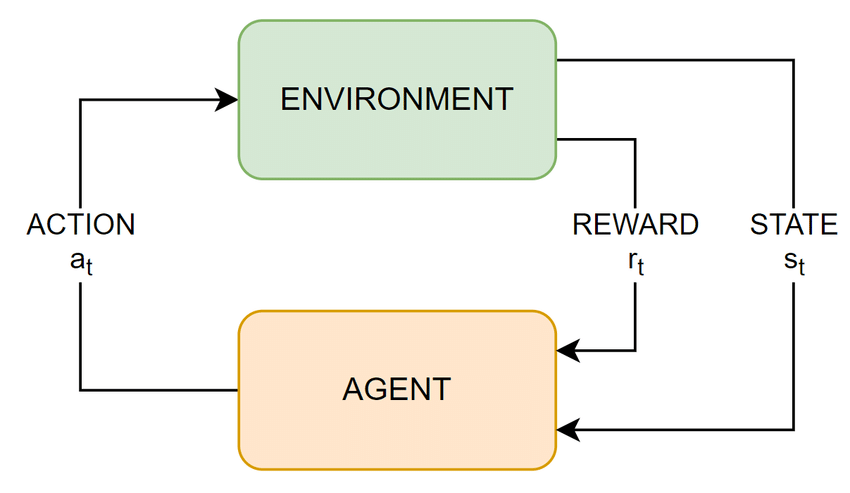
\includegraphics[width=0.5\textwidth]{./figures/Reinforcement-Learning-schema.png}
    \caption{Esquema Reiforcement Learning}
    \label{fig:RF-schema}
\end{figure}

En cada paso de tiempo \(t\), el agente recibe una una observación \(O_t\) y una recompensa \(R_t\).
La observación recibida le permite ejecutar una acción \(A_t\), la cual provocará que el entorno cambie
y emita una nueva observación \(O_{t+1}\) y una nueva recompensa \(R_{t+1}\).

\subsubsection{Hipótesis de la Recompensa}

Una recompensa \(R_t\) es una señal de retroalimentación escalar que indica cómo de buena ha sido la accion 
tomada por el agente en el paso \(t\). 

A partir de esta señal de recopensa se formula
la \textit{hipótesis de la recompensa}, que afirma que en un esquema de aprendizaje por refuerzo, cualquier 
objetivo puede ser formalizado como el resultado de maximizar una recompensa acumulativa. Es decir, el objetivo del agente puede ser expresado como la maximización de una función de recompensa a lo 
largo del tiempo.

Esta función de recompensa se conoce como \textit{retorno} (\(G_t\)), y se define matemáticamente como el sumatorio
de las recompensas futuras, descontadas por un factor de descuento  \(\gamma\):

\[
G_t = R_{t+1} + \gamma R_{t+2} + \gamma^2 R_{t+3} + \dots = \sum_{k=0}^{\infty} \gamma^k R_{t+k+1}
\]
El retorno \(G_t\) es lo que el agente intenta maximizar, y es la base sobre la cual se definen otros elementos como la función de valor.


Esto proporciona un marco ampliamente aplicable en situaciones donde 
las decisiones se toman en una serie de pasos, lo que incluye problemas de control robótico, juegos, 
y \textit{trading} financiero.

En el contexto particular del trading financiero, debido a la naturaleza secuencial y dinámica de 
los mercados, los agentes deben tomar decisiones basadas en información incompleta y en constante 
cambio, buscando maximizar una recompensa a largo plazo, como la rentabilidad de una cartera.

%\subsection{Conceptos Fundamentales de RL}

% \subsubsection{Funciones de Valor}

% La función de valor de un estado \(s\) es el valor esperado del retorno, dado que el agente empieza en ese estado y sigue una política \(\pi\):
% \[
% v(s) = \mathbb{E}[G_t | S_t = s] = \mathbb{E}[R_{t+1} + R_{t+2} + R_{t+3} + \ldots | S_t = s]
% \]
% El objetivo del agente es maximizar esta función de valor, seleccionando acciones que maximicen el valor esperado a largo plazo.

% \subsubsection{Maximización del Valor a través de Acciones}

% El objetivo en RL es seleccionar acciones que maximicen el valor esperado. Esto es crucial porque las acciones pueden tener consecuencias a largo plazo, y la recompensa puede estar retrasada. Es decir, puede ser necesario sacrificar una recompensa inmediata para obtener una mayor recompensa en el futuro.

\subsection{Componentes Básicos del Aprendizaje por Refuerzo}

El aprendizaje por refuerzo se formaliza mediante un \textit{Proceso de Decisión de Markov} (MDP), 
que se define por un cuarteto \(\langle S, A, P, R \rangle\) el cual describe el problema de decisión.

Un MDP se representa por un conjunto de estados \(S\), 
un conjunto de acciones \(A\), una función de transición de estados \(P(s'|s, a)\), y una función de 
recompensa \(R(s, a)\). El objetivo del agente es aprender una política \(\pi(a|s)\) que maximice la 
recompensa acumulada a lo largo del tiempo.

Un proceso de decisión se dice que es Markov si la probabilidad de transición depende únicamente
del estado y acción actuales, no de la historia completa:

\[
p(r, s' | S_t, A_t) = p(r, s' | H_t, A_t)
\]

Esto significa que el estado contiene toda la información relevante de la historia, siendo la historia 
la secuencia completa de observaciones, acciones y recompensas. No quiere decir que la historia contenga
toda la información, sino más bien que el añadir cualquier información adicional no afectará la decisión.

\subsubsection{Estados (\(S\))}
    Representan todas las posibles situaciones en las que se puede encontrar el agente dentro del entorno.
\subsubsection{Política}

Una \textit{política} define el comportamiento del agente, es decir, es un mapeo de estados a acciones. Las políticas pueden ser:
\begin{itemize}
    \item \textbf{Determinísticas}: \(A = \pi(S)\).
    \item \textbf{Estocásticas}: \(\pi(A|S) = p(A|S)\), donde \(A\) es elegido probabilísticamente dado el estado \(S\).
\end{itemize}

\subsubsection{Función de Valor}

En el contexto del RL, las funciones de valor son fundamentales para evaluar qué tan "bueno" es estar en un estado o tomar una acción específica en un estado, bajo una política dada \(\pi\). Existen dos tipos principales de funciones de valor:

\begin{itemize}
    \item \textbf{Función de Valor de Estado (\(V^{\pi}(s)\))}: 
    \[
    V^{\pi}(s) = \mathbb{E}[G_t | S_t = s, \pi] = \mathbb{E}[R_{t+1} + \gamma R_{t+2} + \gamma^2 R_{t+3} + \ldots | S_t = s, \pi]
    \]
    Esta función estima el valor esperado del retorno futuro comenzando desde el estado \(s\) y siguiendo la política \(\pi\).
    
    \item \textbf{Función de Valor de Acción (\(Q^{\pi}(s, a)\))}: 
    \[
    Q^{\pi}(s, a) = \mathbb{E}[G_t | S_t = s, A_t = a, \pi] = \mathbb{E}[R_{t+1} + \gamma R_{t+2} + \gamma^2 R_{t+3} + \ldots | S_t = s, A_t = a, \pi]
    \]
    Esta función estima el valor esperado del retorno futuro al tomar la acción \(a\) en el estado \(s\) y seguir la política \(\pi\) a partir de entonces.
\end{itemize}

El agente usa estas funciones de valor para seleccionar acciones que maximicen el retorno esperado a largo plazo.

\subsubsection{Ecuación de Bellman}

La ecuación de Bellman proporciona una forma recursiva de calcular las funciones de valor, aprovechando la estructura de las recompensas futuras. Para la función de valor de estado, la ecuación de Bellman es:
\[
V^{\pi}(s) = \mathbb{E}[R_{t+1} + \gamma V^{\pi}(S_{t+1}) | S_t = s, \pi]
\]
De manera similar, para la función de valor de acción:
\[
Q^{\pi}(s, a) = \mathbb{E}[R_{t+1} + \gamma Q^{\pi}(S_{t+1}, A_{t+1}) | S_t = s, A_t = a, \pi]
\]
Estas ecuaciones son fundamentales para el desarrollo de algoritmos de RL, ya que permiten descomponer el problema de optimización en subproblemas más manejables.

\subsection{Métodos Clásicos de Aprendizaje por Refuerzo}

Existen varios algoritmos clásicos de RL que permiten a los agentes aprender políticas óptimas, siendo los más conocidos \textit{Q-learning} y \textit{SARSA}.

\begin{itemize}
    \item \textbf{Q-learning}: Un algoritmo \textit{off-policy} que aprende la función de valor de acción \(Q(s, a)\) actualizando iterativamente las estimaciones en función de las recompensas recibidas:
    \[
    Q(s_t, a_t) \leftarrow Q(s_t, a_t) + \alpha \left[r_{t+1} + \gamma \max_{a'} Q(s_{t+1}, a') - Q(s_t, a_t)\right]
    \]
    donde \(\alpha\) es la tasa de aprendizaje. Como algoritmo \textit{off-policy}, Q-learning aprende la política óptima independientemente de la política que el agente sigue durante la exploración. Esto significa que la política utilizada para seleccionar acciones (\textit{behavior policy}) puede ser diferente de la política que se está optimizando (\textit{target policy}).

    \item \textbf{SARSA}: Un algoritmo \textit{on-policy} que, a diferencia de Q-learning, sigue la política actual para actualizar la función \(Q(s, a)\). La actualización en SARSA se realiza utilizando la acción que el agente realmente toma, lo que significa que la política utilizada para seleccionar acciones es la misma que se está optimizando:
    \[
    Q(s_t, a_t) \leftarrow Q(s_t, a_t) + \alpha \left[r_{t+1} + \gamma Q(s_{t+1}, a_{t+1}) - Q(s_t, a_t)\right]
    \]
    Como resultado, SARSA tiende a ser más conservador en su aprendizaje, ya que la política sigue siendo consistente entre el aprendizaje y la ejecución.
\end{itemize}

\subsection{Trade-off Exploración-Explotación}

En el Aprendizaje por Refuerzo, un desafío clave es el equilibrio entre \textit{exploración} y \textit{explotación}. Este balance es fundamental para el aprendizaje efectivo del agente:

\begin{itemize}
    \item \textbf{Exploración}: El agente intenta nuevas acciones para descubrir si existen mejores recompensas disponibles. La exploración es crucial cuando el agente no tiene suficiente conocimiento del entorno y necesita recolectar más información.
    \item \textbf{Explotación}: El agente selecciona la mejor acción conocida basada en su política actual para maximizar la recompensa inmediata. La explotación se basa en la información acumulada y tiene como objetivo maximizar la recompensa a corto plazo.
\end{itemize}

El \textit{trade-off} entre exploración y explotación es crucial porque un agente que explora demasiado podría no aprovechar las recompensas conocidas, mientras que un agente que explota demasiado podría perder oportunidades para descubrir estrategias más efectivas. Existen diversas estrategias para manejar este trade-off, como la \textit{política epsilon-greedy}, donde con una probabilidad \(\epsilon\), el agente explora una acción al azar, y con una probabilidad \(1-\epsilon\), explota la mejor acción conocida. El valor de \(\epsilon\) generalmente disminuye a medida que el agente gana más confianza en su política, lo que permite una mayor explotación con el tiempo.

---


\section{Evolución del Deep Reinforcement Learning (DRL)}

\subsection{Combinación con Redes Neuronales}

El \textit{Deep Reinforcement Learning} (DRL) surge como una evolución natural del \textit{Aprendizaje por Refuerzo} (RL) tradicional, combinando sus principios con la potencia de las redes neuronales profundas (\textit{Deep Learning}). Mientras que los métodos clásicos de RL, como el \textit{Q-learning}, son eficaces en problemas con espacios de estados discretos y de baja dimensionalidad, presentan limitaciones significativas cuando se aplican a entornos complejos y continuos. 

El uso de redes neuronales como aproximadores de funciones en RL permitió superar estas limitaciones. Las redes neuronales profundas son capaces de procesar entradas de alta dimensionalidad y de extraer características complejas directamente de los datos sin la necesidad de diseñar manualmente las características relevantes. Esta capacidad ha sido particularmente útil en problemas de RL donde el espacio de estados es continuo o extremadamente grande, como es común en el trading financiero, la robótica y los videojuegos.

\subsection{Principales Algoritmos de DRL}

El desarrollo de DRL ha dado lugar a una serie de algoritmos innovadores que han transformado la forma en que se aborda el aprendizaje por refuerzo en entornos complejos. A continuación, se presentan algunos de los algoritmos más importantes en este campo:

\subsubsection{Deep Q-Networks (DQN)}

El \textit{Deep Q-Network} (DQN) es uno de los algoritmos más representativos de la combinación entre RL y Deep Learning. DQN fue introducido por \textit{DeepMind} y marcó un hito en la historia del RL al aplicar redes neuronales profundas para aproximar la función \(Q(s, a)\), lo que permitió manejar entornos con espacios de estados grandes y continuos.

En DQN, una red neuronal recibe como entrada el estado del entorno y produce una estimación de los valores \(Q(s, a)\) para cada acción posible. La red se entrena utilizando el algoritmo de \textit{Q-learning} tradicional, pero con varias modificaciones clave para estabilizar el aprendizaje, como el uso de un \textit{buffer} de \textit{replay} para almacenar transiciones de experiencias pasadas y el uso de una red objetivo (\textit{target network}) que se actualiza periódicamente para reducir la inestabilidad en la actualización de los valores \(Q\).

\subsubsection{Policy Gradient Methods}

Los \textit{Policy Gradient Methods} son un enfoque alternativo en DRL, en el cual en lugar de aprender una función de valor, el agente aprende directamente una política parametrizada \(\pi_{\theta}(a|s)\) que maximiza la recompensa esperada. La principal ventaja de los métodos de gradiente de política es su capacidad para manejar espacios de acción continuos y para aprender políticas estocásticas.

Un algoritmo básico dentro de esta categoría es \textit{REINFORCE}, que utiliza el gradiente de la recompensa esperada para actualizar los parámetros de la política. Aunque REINFORCE es sencillo y conceptualmente atractivo, su principal limitación es la alta varianza en las estimaciones del gradiente, lo que puede llevar a un aprendizaje lento y inestable.

\subsubsection{Actor-Critic Methods}

Los métodos \textit{Actor-Critic} combinan lo mejor de ambos mundos al utilizar tanto una función de valor como una política parametrizada. En este enfoque, el \textit{actor} es responsable de seleccionar las acciones basadas en la política \(\pi_{\theta}(a|s)\), mientras que el \textit{crítico} estima el valor de la política actual utilizando una función de valor \(V^{\pi}(s)\) o \(Q^{\pi}(s, a)\). 

Un ejemplo notable es el \textit{Asynchronous Advantage Actor-Critic} (A3C), que introduce el concepto de ventaja (\textit{advantage}), definida como la diferencia entre el valor de la acción y el valor esperado del estado (\(A(s, a) = Q(s, a) - V(s)\)). A3C mejora la estabilidad del aprendizaje al usar múltiples actores que interactúan con copias del entorno en paralelo, lo que también mejora la eficiencia computacional.

\subsection{Avances y Limitaciones}

El desarrollo del DRL ha permitido avances significativos en la capacidad de los agentes para aprender en entornos complejos y de alta dimensionalidad. Algunos de los avances más destacados incluyen:

\begin{itemize}
    \item \textbf{Escalabilidad}: El uso de redes neuronales profundas ha permitido que los algoritmos de RL escalen a problemas que antes eran inabordables, como juegos complejos y mercados financieros.
    \item \textbf{Capacidad de Generalización}: DRL ha mostrado una notable capacidad para generalizar el conocimiento adquirido en un entorno a otros entornos similares, lo que es crucial en aplicaciones como el trading, donde las condiciones del mercado cambian constantemente.
    \item \textbf{Desempeño en Tareas Complejas}: DRL ha superado a los humanos en varias tareas complejas, como juegos de Atari, y ha logrado una eficiencia sin precedentes en aplicaciones como la optimización de portafolios.
\end{itemize}

Sin embargo, el DRL también presenta limitaciones que deben ser abordadas:

\begin{itemize}
    \item \textbf{Complejidad Computacional}: Entrenar modelos de DRL requiere un poder computacional significativo y grandes volúmenes de datos, lo que puede ser un obstáculo para su aplicación en tiempo real.
    \item \textbf{Estabilidad y Convergencia}: Los algoritmos de DRL pueden ser inestables y propensos a la divergencia durante el entrenamiento, especialmente en entornos con recompensas escasas o en problemas altamente no lineales.
    \item \textbf{Sensibilidad a la Parametrización}: El desempeño de los algoritmos de DRL es altamente sensible a la elección de hiperparámetros, lo que requiere una considerable experimentación y ajuste fino.
\end{itemize}

En conclusión, el DRL ha ampliado significativamente el alcance de las aplicaciones de RL, permitiendo a los agentes abordar problemas más complejos y realistas. No obstante, sigue siendo un área de investigación activa con desafíos técnicos y prácticos que deben ser resueltos para su adopción generalizada.


PUNTOS A INTRODUCIIIIIIIIIIIIIIR
\begin{itemize}
   \item Explicación de las ecuaciones y metodos ( bellman, metodos de diferencias temporales vs monte carlo, )
   \item Algoritmos utilizados
   \item Implementación del entorno en gimnasium
   \item obtención del espacio de observaciones (indicadores...)
   \item funciones de recompensa
   \item resultados
   \item conclusiones
\end{itemize}

\chapter{Meta-labeling}

Consiste en la utilización de un modelo secundario para afinar las predicciones del primario.

\begin{itemize}
   \item \textbf{Generación de señales}: El modelo primario genera señales
   \item \textbf{Asignación de labeles}: Cada señal generada por el modelo primario se etiqueta como correcta o incorrecta en base al rendimiento observado.
   \item El libro propone varias maneras de hacerlo.
   \item \textbf{Entrenamiento del meta-modelo}: El meta-modelo se entrena utilizando estas etiquetas y otras features adicionales que puedan influir en la precision de la señla.
   \item \textbf{Prediccion de la calidad de la señales}: Una vez entrenado, el meta-modelo se utiliza para predecir la probabilidad de que las 
   futuras señales del modelo primario sean correctas.
\end{itemize}

\chapter{Conclusiones}

\appendix

\chapter{Demostración del teorema}

%\phantomsection
%\addcontentsline{toc}{chapter}{BIBLIOGRAFIA}
\bibliographystyle{plain}
\bibliography{biblioTFM}

\end{document}